% =============================================================
% NutriTrack — Certification Defense Slides (Visual Edition)
% RNCP37638 — Expert in Massive Data Infrastructures
% ~45 slides — visual, less text, clear workflow
% =============================================================
\documentclass[aspectratio=169, 10pt]{beamer}

\usetheme{metropolis}
\metroset{progressbar=frametitle, numbering=fraction, block=fill, sectionpage=progressbar}

% ── Colors ────────────────────────────────────────────────────
\definecolor{ntgreen}{HTML}{2E7D32}
\definecolor{ntlightgreen}{HTML}{66BB6A}
\definecolor{ntdarkgreen}{HTML}{1B5E20}
\definecolor{ntbg}{HTML}{FAFAFA}
\definecolor{ntaccent}{HTML}{FF8F00}
\definecolor{ntblue}{HTML}{1565C0}
\definecolor{ntred}{HTML}{C62828}
\definecolor{ntpurple}{HTML}{6A1B9A}
\definecolor{bronze}{HTML}{CD7F32}
\definecolor{silver}{HTML}{A0A0A0}
\definecolor{gold}{HTML}{DAA520}
\definecolor{demobox}{HTML}{FFF3E0}
\definecolor{whybox}{HTML}{E3F2FD}
\definecolor{vsbox}{HTML}{FFF8E1}

\setbeamercolor{palette primary}{bg=ntgreen, fg=white}
\setbeamercolor{frametitle}{bg=ntgreen, fg=white}
\setbeamercolor{progress bar}{fg=ntaccent, bg=ntgreen!20}
\setbeamercolor{title separator}{fg=ntaccent}
\setbeamercolor{alerted text}{fg=ntaccent}
\setbeamercolor{example text}{fg=ntgreen}
\setbeamercolor{block title}{bg=ntgreen, fg=white}
\setbeamercolor{block body}{bg=ntgreen!5}
\setbeamercolor{block title alerted}{bg=ntred, fg=white}
\setbeamercolor{block body alerted}{bg=ntred!5}

% ── Packages ──────────────────────────────────────────────────
\usepackage[english]{babel}
\usepackage{tikz}
\usetikzlibrary{arrows.meta, positioning, shapes.geometric, calc, fit,
  decorations.pathreplacing, decorations.text, backgrounds, matrix, shadows}
\usepackage{fontawesome5}
\usepackage{booktabs}
\usepackage{graphicx}
\usepackage{listings}
\usepackage{multicol}
\usepackage{xcolor}
\usepackage{hyperref}

\lstset{
  basicstyle=\tiny\ttfamily, breaklines=true, frame=single,
  backgroundcolor=\color{ntbg},
  keywordstyle=\color{ntblue}\bfseries,
  commentstyle=\color{gray}, stringstyle=\color{ntgreen},
}

% ── Custom commands ───────────────────────────────────────────
\newcommand{\nutritrack}{\textsc{NutriTrack}}
\newcommand{\competency}[1]{\textbf{\color{ntblue}#1}}
\newcommand{\fullcov}{\textcolor{ntgreen}{\faCheckCircle}}

\newcommand{\democallout}[1]{%
  \begin{center}\begin{tikzpicture}
    \node[fill=demobox, rounded corners=8pt, inner sep=8pt,
          draw=ntaccent, line width=1.5pt]
      {\large\faDesktop\;\textbf{\color{ntaccent}LIVE DEMO:} #1};
  \end{tikzpicture}\end{center}}

\newcommand{\whycallout}[1]{%
  \begin{center}\begin{tikzpicture}
    \node[fill=whybox, rounded corners=6pt, inner sep=6pt,
          draw=ntblue!50, line width=1pt, text width=0.92\linewidth]
      {\small\faLightbulb\;\textbf{\color{ntblue}Why?} #1};
  \end{tikzpicture}\end{center}}

% NutriTrack logo command (scalable)
\newcommand{\nutritracklogo}[1][1]{%
\begin{tikzpicture}[scale=#1, transform shape]
  % Outer circle
  \fill[ntgreen] (0,0) circle (1.3);
  \fill[ntdarkgreen] (0,0) circle (1.15);
  % Inner ring
  \draw[white, line width=1.5pt] (0,0) circle (1.0);
  % Fork icon (left)
  \fill[white] (-0.35,0.55) -- (-0.35,-0.15) -- (-0.42,-0.15)
    arc (180:0:0.07) -- (-0.28,-0.15) -- (-0.28,0.55)
    arc (0:180:0.035) -- cycle;
  \fill[white] (-0.35,-0.15) -- (-0.35,-0.65)
    arc (180:360:0.035) -- (-0.28,-0.15) -- cycle;
  % Leaf icon (right, simplified)
  \fill[ntlightgreen] (0.3,0.05)
    .. controls (0.55,0.55) and (0.15,0.7) .. (0.1,0.45)
    .. controls (0.08,0.25) and (0.15,-0.05) .. (0.3,0.05) -- cycle;
  \draw[white, line width=0.6pt] (0.25,0.1) .. controls (0.22,0.3) .. (0.18,0.45);
  \draw[white, line width=0.4pt] (0.22,0.25) -- (0.32,0.35);
  \draw[white, line width=0.4pt] (0.20,0.35) -- (0.12,0.28);
  % NT text
  \node[font=\bfseries\large, text=white] at (0,-0.45) {NT};
  % Outer label arc (top)
  \path[decorate, decoration={text along path,
    text={|\tiny\bfseries\color{white}|NUTRITRACK},
    text align=center, raise=0pt}]
    (140:1.05) arc (140:40:1.05);
\end{tikzpicture}%
}

% ── Title ─────────────────────────────────────────────────────
\title{\nutritrack}
\subtitle{Nutritional Data Engineering Platform}
\author{Reetika Gautam}
\date{April 2026}
\institute{RNCP37638 --- Expert in Massive Data Infrastructures\\
  Level 7 (Master's equivalent) \;\textbullet\; Simplon.co}

\begin{document}

% ======================= SLIDE 1: TITLE =======================
\begin{frame}[standout]
  \vspace*{-0.8cm}
  \nutritracklogo[1.3]\\[0.4cm]
  {\Huge\bfseries \nutritrack}\\[0.3cm]
  {\large Nutritional Data Engineering Platform}\\[0.6cm]
  {\normalsize Reetika Gautam}\\[0.15cm]
  {\small RNCP37638 --- Expert in Massive Data Infrastructures}\\
  {\small Level 7 $\bullet$ April 2026 $\bullet$ Simplon.co}
\end{frame}

% ======================= SLIDE 2: AGENDA ======================
\begin{frame}{Defense Agenda --- 90 Minutes}
\begin{center}

\begin{tikzpicture}[scale=0.85, transform shape,
  block/.style={rounded corners=8pt, minimum width=2.8cm, minimum height=1.2cm,
                draw, very thick, font=\small\bfseries, align=center, text=white},
  time/.style={font=\scriptsize\bfseries, text=gray}
]
  \node[block, fill=ntgreen] (e15) at (0,0) {E1--E5\\{\scriptsize Project \&}\\{\scriptsize Implementation}};
  \node[block, fill=ntblue] (e6) at (4.2,0) {E6\\{\scriptsize DW Maintenance}\\{\scriptsize Q\&A}};
  \node[block, fill=ntpurple] (e7) at (8.4,0) {E7\\{\scriptsize Data Lake}};
  \node[block, fill=ntaccent] (qa) at (12.2,0) {Jury\\{\scriptsize Questions}};
  \node[time] at (0,-1) {60 min};
  \node[time] at (4.2,-1) {10 min};
  \node[time] at (8.4,-1) {10 min};
  \node[time] at (12.2,-1) {10 min};
  \draw[-{Stealth}, very thick, gray!50] (e15) -- (e6);
  \draw[-{Stealth}, very thick, gray!50] (e6) -- (e7);
  \draw[-{Stealth}, very thick, gray!50] (e7) -- (qa);
  \node[font=\tiny, ntgreen!70] at (0,1) {C1--C15};
  \node[font=\tiny, ntblue!70] at (4.2,1) {C16--C17};
  \node[font=\tiny, ntpurple!70] at (8.4,1) {C18--C21};
\end{tikzpicture}
\end{center}
\vspace{0.3cm}
\begin{center}
  {\footnotesize\faDesktop\ \textbf{Live demos} throughout $\bullet$
   \faFile*\ Report handed to jury $\bullet$
   \faGithub\ Code on GitHub}
\end{center}
\end{frame}

% ======================= SLIDE 3: THE CLIENT ===================
\begin{frame}{Meet the Client --- Ms.\ Sophie Yang}
\begin{columns}[T]
\begin{column}{0.45\textwidth}
  \begin{center}
  \begin{tikzpicture}
    \node[circle, fill=ntgreen!15, draw=ntgreen, very thick,
          minimum size=2.5cm, font=\Huge] {\faUserMd};
    \node[font=\normalsize\bfseries, ntgreen] at (0,-2) {Ms.\ Sophie Yang};
    \node[font=\scriptsize] at (0,-2.5) {Dietician --- Paris};
    \node[font=\scriptsize, gray] at (0,-3) {40+ patients/week};
  \end{tikzpicture}
  \end{center}
\end{column}
\begin{column}{0.52\textwidth}
  \begin{tikzpicture}[
    pain/.style={rounded corners=5pt, fill=ntred!8, draw=ntred, thick,
                 minimum width=4.5cm, minimum height=0.7cm, align=left,
                 font=\scriptsize, inner xsep=6pt},
  ]
    \node[font=\small\bfseries, ntred] at (0,2.5) {\faExclamationTriangle\ Her daily pain points};
    \node[pain] at (0,1.7) {\faSearch\ Manually searches Open Food Facts};
    \node[pain] at (0,0.9) {\faTable\ Calculates macros in spreadsheets};
    \node[pain] at (0,0.1) {\faChartLine\ Cannot track patient progress};
    \node[pain] at (0,-0.7) {\faRandom\ Data scattered across 5+ sources};
    \node[pain] at (0,-1.5) {\faTimesCircle\ No RGPD compliance for health data};
  \end{tikzpicture}
\end{column}
\end{columns}

\vspace{0.3cm}
\begin{center}
  {\large\color{ntred}\textit{``I spend hours looking up products. I need a platform\\
  where my patients log meals and I see the analytics.''}}
\end{center}

\note{
  Introduce Sophie Yang, the client. Her pain points drive every feature.
  This is C1: analyzing a data project need expression.
}
\end{frame}

% =============================================================
\section{E1 --- Need Analysis (C1)}
% =============================================================

% ======================= SLIDE 4: INTERVIEW GRIDS ============
\begin{frame}{Interview Grids \competency{C1}}
\begin{center}
\begin{tikzpicture}[
  card/.style={rounded corners=6pt, minimum width=5.2cm, minimum height=4.2cm,
               draw, thick, align=left, font=\scriptsize, inner sep=8pt},
  icon/.style={circle, minimum size=0.8cm, font=\large, text=white},
]
  \node[card, fill=ntgreen!5, draw=ntgreen] (prod) at (-3.5,0) {};
  \node[icon, fill=ntgreen] at (-3.5,2.5) {\faUsers};
  \node[font=\small\bfseries, ntgreen] at (-3.5,1.7) {Data Producers};
  \node[font=\scriptsize, text width=4.5cm] at (-3.5,-0.2) {
    \faIndustry\ Business activities\\[1pt]
    \faFile\ Data types \& formats\\[1pt]
    \faTachometerAlt\ Volumes \& frequency\\[1pt]
    \faShieldAlt\ Quality controls\\[1pt]
    \faTags\ Metadata available\\[1pt]
    \faLock\ Access constraints\\[1pt]
    \faExclamationTriangle\ Known issues
  };

  \node[card, fill=ntblue!5, draw=ntblue] (cons) at (3.5,0) {};
  \node[icon, fill=ntblue] at (3.5,2.5) {\faChartBar};
  \node[font=\small\bfseries, ntblue] at (3.5,1.7) {Data Consumers};
  \node[font=\scriptsize, text width=4.5cm] at (3.5,-0.2) {
    \faBullseye\ Analysis objectives\\[1pt]
    \faSearchPlus\ Required granularity\\[1pt]
    \faFileExport\ Delivery format needs\\[1pt]
    \faClock\ Frequency needs\\[1pt]
    \faUserShield\ RGPD constraints\\[1pt]
    \faTools\ Tool preferences\\[1pt]
    \faUniversalAccess\ Accessibility needs
  };
\end{tikzpicture}
\end{center}
\end{frame}

% ======================= SLIDE 5: SMART ======================
\begin{frame}{SMART Objectives \competency{C1}}
\begin{center}
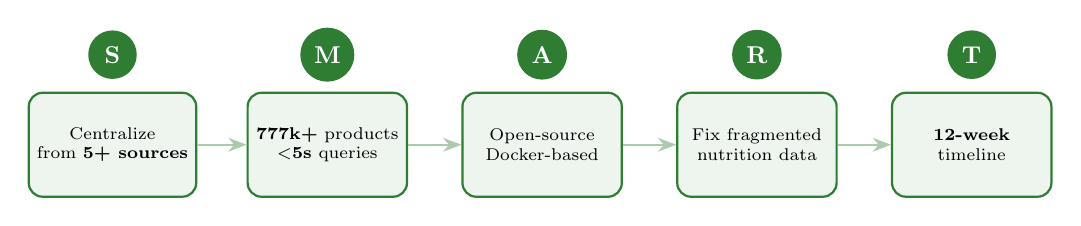
\begin{tikzpicture}[scale=0.88, transform shape,
  smart/.style={rounded corners=5pt, minimum width=2.3cm, minimum height=1.5cm,
                draw=ntgreen, thick, fill=ntgreen!8, align=center, font=\scriptsize},
  letter/.style={circle, fill=ntgreen, text=white, font=\normalsize\bfseries, minimum size=0.7cm},
]
  \node[smart] (s) at (0,0) {Centralize\\from \textbf{5+ sources}};
  \node[smart] (m) at (3.1,0) {\textbf{777k+} products\\$<$\textbf{5s} queries};
  \node[smart] (a) at (6.2,0) {Open-source\\Docker-based};
  \node[smart] (r) at (9.3,0) {Fix fragmented\\nutrition data};
  \node[smart] (t) at (12.4,0) {\textbf{12-week}\\timeline};
  \node[letter] at (0,1.3) {S};
  \node[letter] at (3.1,1.3) {M};
  \node[letter] at (6.2,1.3) {A};
  \node[letter] at (9.3,1.3) {R};
  \node[letter] at (12.4,1.3) {T};
  \draw[-{Stealth}, thick, ntgreen!40] (s)--(m);
  \draw[-{Stealth}, thick, ntgreen!40] (m)--(a);
  \draw[-{Stealth}, thick, ntgreen!40] (a)--(r);
  \draw[-{Stealth}, thick, ntgreen!40] (r)--(t);
\end{tikzpicture}
\end{center}
\vspace{0.2cm}
\begin{center}
\begin{tikzpicture}
  \node[rounded corners=8pt, fill=ntblue!5, draw=ntblue!40, inner sep=8pt,
        text width=0.92\linewidth, font=\small] {
    \textbf{Pre-project:}\quad
    \faFile*\ Technical recommendations \quad
    \faUserShield\ RGPD actions \quad
    \faUniversalAccess\ Accessibility planned \quad
    \faSortAmountDown\ RICE prioritization
  };
\end{tikzpicture}
\end{center}
\end{frame}

% ======================= SLIDE 6: SOLUTION ====================
\begin{frame}{NutriTrack --- Built for Sophie}
\begin{center}
\begin{tikzpicture}[
  need/.style={rounded corners=6pt, fill=ntred!8, draw=ntred, thick,
               minimum width=4.5cm, minimum height=1.2cm, align=center, font=\scriptsize},
  sol/.style={rounded corners=6pt, fill=ntgreen!8, draw=ntgreen, thick,
              minimum width=4.5cm, minimum height=1.2cm, align=center, font=\scriptsize},
]
  \node[font=\small\bfseries, ntred] at (-3.5,2.2) {Sophie's Need};
  \node[font=\small\bfseries, ntgreen] at (3.5,2.2) {What We Built};

  \node[need] (n1) at (-3.5,1.1) {``I search products manually\\across multiple sites''};
  \node[sol]  (s1) at (3.5,1.1) {\faDownload\ 5 automated extractors\\+ unified product search};

  \node[need] (n2) at (-3.5,-0.3) {``I can't track patient\\meals over time''};
  \node[sol]  (s2) at (3.5,-0.3) {\faUtensils\ Meal logger + daily dashboard\\+ weekly trends};

  \node[need] (n3) at (-3.5,-1.7) {``Patient data is sensitive\\--- I worry about compliance''};
  \node[sol]  (s3) at (3.5,-1.7) {\faShieldAlt\ Full RGPD: consent, registry,\\auto-cleanup, pseudonymization};

  \draw[-{Stealth}, very thick, ntaccent] (n1) -- (s1);
  \draw[-{Stealth}, very thick, ntaccent] (n2) -- (s2);
  \draw[-{Stealth}, very thick, ntaccent] (n3) -- (s3);
\end{tikzpicture}
\end{center}

\vspace{0.1cm}
\begin{center}
\begin{tikzpicture}
  \node[rounded corners=8pt, fill=ntgreen!5, draw=ntgreen!40,
        inner sep=8pt, font=\small] {
    \faDatabase\ \textbf{777k+} products \quad
    \faDocker\ \textbf{14} services \quad
    \faCogs\ \textbf{7} DAGs \quad
    \faUsers\ \textbf{4} roles \quad
    \faTerminal\ \textbf{1} command to deploy
  };
\end{tikzpicture}
\end{center}

\note{
  Every technical choice maps back to Sophie's needs.
  This is the core narrative of the entire defense.
}
\end{frame}

% ======================= SLIDE 5: OPEN FOOD FACTS ==============
\begin{frame}{Open Food Facts --- Our Primary Data Source}
\begin{columns}[T]
\begin{column}{0.48\textwidth}
  \begin{tikzpicture}
    \node[rounded corners=8pt, fill=ntgreen!5, draw=ntgreen, thick, inner sep=8pt,
          text width=4.5cm, font=\scriptsize, align=left] {
      \textbf{\normalsize\color{ntgreen} Open Food Facts}\\[6pt]
      \faGlobe\ \textbf{French non-profit} founded in 2012\\[3pt]
      \faUsers\ Community of 30{,}000+ contributors\\[3pt]
      \faDatabase\ \textbf{3{,}000{,}000+} food products worldwide\\[3pt]
      \faBalanceScale\ Open Database License (ODbL)\\[3pt]
      \faFlag\ Headquartered in Paris, France\\[6pt]
      \textbf{Mission:} Make food product information\\
      transparent and accessible to everyone.\\[3pt]
      \textbf{Used by:} Yuka, Foodvisor, government\\
      agencies, academic research
    };
  \end{tikzpicture}
\end{column}
\begin{column}{0.48\textwidth}
  \begin{tikzpicture}[
    feat/.style={rounded corners=4pt, minimum width=4.3cm, minimum height=0.55cm,
                 fill=ntblue!8, draw=ntblue!40, font=\scriptsize, align=left, inner xsep=5pt},
  ]
    \node[font=\small\bfseries, ntblue] at (0,3) {What OFF provides};
    \node[feat] at (0,2.2) {\faAppleAlt\ Nutri-Score (A to E) --- nutrition quality};
    \node[feat] at (0,1.4) {\faIndustry\ NOVA group (1--4) --- processing level};
    \node[feat] at (0,0.6) {\faLeaf\ Eco-Score --- environmental impact};
    \node[feat] at (0,-0.2) {\faBarcode\ Barcode identification (EAN-13)};
    \node[feat] at (0,-1.0) {\faList\ Full ingredient lists};
    \node[feat] at (0,-1.8) {\faExclamationTriangle\ Allergen declarations};
    \node[feat] at (0,-2.6) {\faTags\ 31 nutritional fields per product};
  \end{tikzpicture}
\end{column}
\end{columns}

\note{
  OFF is a French NGO. Emphasize: open data, transparency, community-driven.
  Nutri-Score is a French invention now adopted across Europe.
  This is WHY we chose OFF --- it aligns with Sophie's need for trusted nutritional data.
}
\end{frame}

% ======================= SLIDE 6: OFF DATA FORMATS ============
\begin{frame}{OFF Data --- Formats \& What We Extract}
\begin{columns}[T]
\begin{column}{0.48\textwidth}
  \begin{center}
  {\small\textbf{Two access methods}}\\[0.3cm]
  \begin{tikzpicture}[
    method/.style={rounded corners=6pt, minimum width=4.3cm, minimum height=2.2cm,
                   draw, thick, align=left, font=\scriptsize, inner sep=6pt},
  ]
    \node[method, fill=ntgreen!8, draw=ntgreen] at (0,1.8) {
      \faGlobe\ \textbf{REST API} (daily)\\[3pt]
      Endpoint: search.pl?json=1\\
      5 categories searched:\\
      cereals, yogurts, chocolate,\\
      beverages, snacks\\
      Rate-limited: 0.6s between calls\\
      \textbf{Output:} JSON $\sim$1{,}000 products/day
    };
    \node[method, fill=ntblue!8, draw=ntblue] at (0,-1.5) {
      \faFile\ \textbf{Parquet Bulk Export} (weekly)\\[3pt]
      Full OFF dump from HuggingFace\\
      3M+ products in one file\\
      Filtered: country = France\\
      \textbf{Output:} Parquet $\sim$798{,}000 products
    };
  \end{tikzpicture}
  \end{center}
\end{column}
\begin{column}{0.48\textwidth}
  \begin{center}
  {\small\textbf{31 fields per product --- example}}\\[0.3cm]
  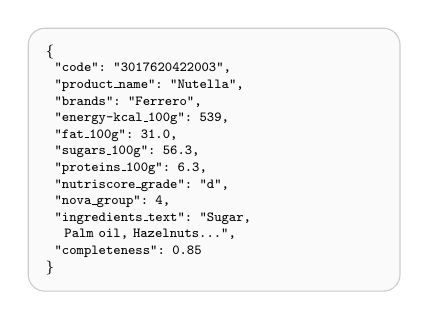
\begin{tikzpicture}
    \node[rounded corners=6pt, fill=ntbg, draw=gray!40, inner sep=6pt,
          text width=4.3cm, font=\tiny\ttfamily, align=left] {
      \{\\
      ~~"code": "3017620422003",\\
      ~~"product\_name": "Nutella",\\
      ~~"brands": "Ferrero",\\
      ~~"energy-kcal\_100g": 539,\\
      ~~"fat\_100g": 31.0,\\
      ~~"sugars\_100g": 56.3,\\
      ~~"proteins\_100g": 6.3,\\
      ~~"nutriscore\_grade": "d",\\
      ~~"nova\_group": 4,\\
      ~~"ingredients\_text": "Sugar,\\
      ~~~~Palm oil, Hazelnuts...",\\
      ~~"completeness": 0.85\\
      \}
    };
  \end{tikzpicture}

  \vspace{0.2cm}
  {\scriptsize\color{gray} Real example: Nutella (barcode 3017620422003)}
  \end{center}
\end{column}
\end{columns}

\note{
  Show the raw data format. Emphasize: 31 fields, but messy ---
  inconsistent naming, missing values, duplicates. That's why we clean it.
}
\end{frame}

% ======================= SLIDE 7: CLEANING EXAMPLES ===========
\begin{frame}{Data Cleaning --- Before \& After \competency{C10}}
\begin{center}
{\small\textbf{7 cleaning rules applied by PySpark in \texttt{aggregate\_clean.py}}}\\[0.15cm]
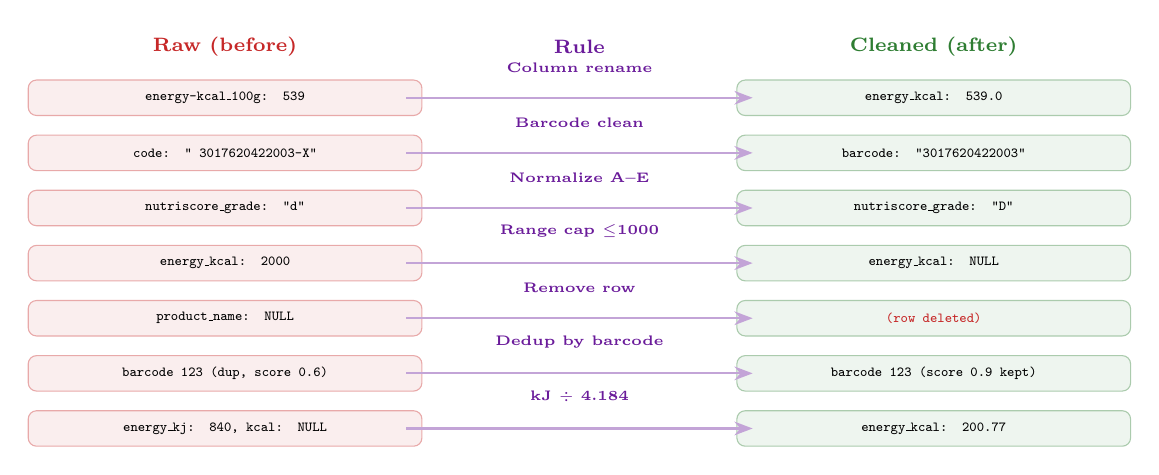
\begin{tikzpicture}[
  raw/.style={rounded corners=3pt, fill=ntred!8, draw=ntred!40,
              minimum width=5cm, minimum height=0.45cm, font=\tiny\ttfamily, align=left, inner xsep=5pt},
  clean/.style={rounded corners=3pt, fill=ntgreen!8, draw=ntgreen!40,
                minimum width=5cm, minimum height=0.45cm, font=\tiny\ttfamily, align=left, inner xsep=5pt},
  rule/.style={font=\tiny\bfseries, ntpurple, text width=2.5cm, align=center},
]
  \node[font=\scriptsize\bfseries, ntred] at (-4.5,2.8) {Raw (before)};
  \node[font=\scriptsize\bfseries, ntgreen] at (4.5,2.8) {Cleaned (after)};
  \node[font=\scriptsize\bfseries, ntpurple] at (0,2.8) {Rule};

  \node[raw]   at (-4.5,2.15) {energy-kcal\_100g: 539};
  \node[rule, above]  at (0,2.35) {Column rename};
  \node[clean] at (4.5,2.15) {energy\_kcal: 539.0};

  \node[raw]   at (-4.5,1.45) {code: " 3017620422003-X"};
  \node[rule, above]  at (0,1.65) {Barcode clean};
  \node[clean] at (4.5,1.45) {barcode: "3017620422003"};

  \node[raw]   at (-4.5,0.75) {nutriscore\_grade: "d"};
  \node[rule, above]  at (0,0.95) {Normalize A--E};
  \node[clean] at (4.5,0.75) {nutriscore\_grade: "D"};

  \node[raw]   at (-4.5,0.05) {energy\_kcal: 2000};
  \node[rule, above]  at (0,0.25) {Range cap $\leq$1000};
  \node[clean] at (4.5,0.05) {energy\_kcal: NULL};

  \node[raw]   at (-4.5,-0.65) {product\_name: NULL};
  \node[rule, above]  at (0,-0.45) {Remove row};
  \node[clean] at (4.5,-0.65) {\color{ntred}(row deleted)};

  \node[raw]   at (-4.5,-1.35) {barcode 123 (dup, score 0.6)};
  \node[rule, above]  at (0,-1.15) {Dedup by barcode};
  \node[clean] at (4.5,-1.35) {barcode 123 (score 0.9 kept)};

  \node[raw]   at (-4.5,-2.05) {energy\_kj: 840, kcal: NULL};
  \node[rule, above]  at (0,-1.85) {kJ $\div$ 4.184};
  \node[clean] at (4.5,-2.05) {energy\_kcal: 200.77};

  % Arrows
  \foreach \y in {2.15,1.45,0.75,0.05,-0.65,-1.35,-2.05}
    \draw[-{Stealth}, thick, ntpurple!40] (-2.2,\y) -- (2.2,\y);
\end{tikzpicture}
\end{center}
\vspace{-0.1cm}
{\scriptsize\textbf{Result:} 798{,}177 raw $\to$ 777{,}126 clean products (2.6\% removal rate). Output: \texttt{products\_cleaned.parquet}}

\note{
  C10: Walk through each rule with the visual.
  Emphasize: physiological max cap prevents impossible values.
  Dedup keeps the most complete record per barcode.
}
\end{frame}

% ======================= SLIDE 8: END-TO-END FLOW =============
\begin{frame}{End-to-End Data Flow}
\begin{center}
\begin{tikzpicture}[scale=0.85, transform shape,
  stepnode/.style={rounded corners=6pt, minimum width=2cm, minimum height=1.2cm,
               draw, very thick, align=center, font=\scriptsize},
]
  \node[stepnode, fill=ntgreen!12, draw=ntgreen] (ext) at (0,0) {\faDownload\\Extract\\{\tiny 5 scripts}};
  \node[stepnode, fill=ntaccent!12, draw=ntaccent] (raw) at (3,0) {\faFolder\\Raw Files\\{\tiny /data/raw/}};
  \node[stepnode, fill=ntpurple!12, draw=ntpurple] (cln) at (6,0) {\faFilter\\Clean\\{\tiny aggregate\_clean}};
  \node[stepnode, fill=ntblue!12, draw=ntblue] (app) at (9,0) {\faDatabase\\App DB\\{\tiny PostgreSQL}};

  \node[stepnode, fill=ntblue!12, draw=ntblue] (dw) at (6,-2.5) {\faStar\\Warehouse\\{\tiny Star schema}};
  \node[stepnode, fill=bronze!12, draw=bronze] (lake) at (12,-2.5) {\faCloud\\Data Lake\\{\tiny Medallion}};

  \node[stepnode, fill=ntaccent!12, draw=ntaccent] (api) at (3,-2.5) {\faPlug\\FastAPI\\{\tiny REST}};
  \node[stepnode, fill=ntaccent!12, draw=ntaccent] (stl) at (3,-4.5) {\faDesktop\\Streamlit\\{\tiny 4 roles}};
  \node[stepnode, fill=ntred!12, draw=ntred] (mon) at (9,-4.5) {\faChartLine\\Grafana\\{\tiny Monitoring}};

  \draw[-{Stealth}, very thick, ntgreen!50] (ext) -- (raw);
  \draw[-{Stealth}, very thick, ntaccent!50] (raw) -- (cln);
  \draw[-{Stealth}, very thick, ntpurple!50] (cln) -- (app);
  \draw[-{Stealth}, very thick, ntblue!50] (app) -- (dw);
  \draw[-{Stealth}, very thick, ntblue!50] (app.east) -- ++(0.5,0) |- (lake);
  \draw[-{Stealth}, very thick, ntblue!50] (app) -- (api);
  \draw[-{Stealth}, very thick, ntaccent!50] (api) -- (stl);
  \draw[-{Stealth}, very thick, ntblue!50] (dw.south) -- ++(0,-1) -| (stl);

  % Labels
  \node[font=\tiny\bfseries, ntgreen] at (1.5,0.5) {02:00};
  \node[font=\tiny\bfseries, ntpurple] at (4.5,0.5) {04:00};
  \node[font=\tiny\bfseries, ntblue] at (7.5,0.5) {04:30};
  \node[font=\tiny\bfseries, ntblue] at (7.5,-1.5) {05:00};

  % Users
  \node[font=\tiny] at (3,-5.3) {\faUser\ Users / Nutritionists / Analysts};
  \node[font=\tiny] at (9,-5.3) {\faUserCog\ Ops team};
\end{tikzpicture}
\end{center}
\end{frame}

% ======================= SLIDE 6: DOCKER EXPLAINED ============
\begin{frame}{One Command, 14 Services}
\begin{center}
  {\large\ttfamily\color{ntgreen} docker compose up -d}\\[0.4cm]
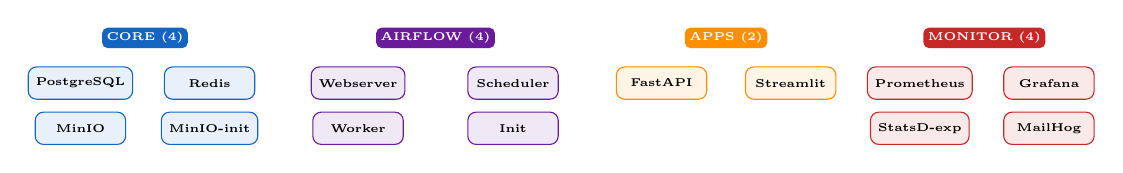
\begin{tikzpicture}[scale=0.82, transform shape,
  svc/.style={rounded corners=3pt, minimum width=1.4cm, minimum height=0.5cm,
              draw, font=\tiny\bfseries, align=center},
  cat/.style={font=\tiny\bfseries, text=white, rounded corners=2pt, inner sep=2pt},
]
  % Categories
  \node[cat, fill=ntblue] at (-1.5,2.5) {CORE (4)};
  \node[svc, fill=ntblue!10, draw=ntblue] at (-2.5,1.8) {PostgreSQL};
  \node[svc, fill=ntblue!10, draw=ntblue] at (-0.5,1.8) {Redis};
  \node[svc, fill=ntblue!10, draw=ntblue] at (-2.5,1.1) {MinIO};
  \node[svc, fill=ntblue!10, draw=ntblue] at (-0.5,1.1) {MinIO-init};

  \node[cat, fill=ntpurple] at (3,2.5) {AIRFLOW (4)};
  \node[svc, fill=ntpurple!10, draw=ntpurple] at (1.8,1.8) {Webserver};
  \node[svc, fill=ntpurple!10, draw=ntpurple] at (4.2,1.8) {Scheduler};
  \node[svc, fill=ntpurple!10, draw=ntpurple] at (1.8,1.1) {Worker};
  \node[svc, fill=ntpurple!10, draw=ntpurple] at (4.2,1.1) {Init};

  \node[cat, fill=ntaccent] at (7.5,2.5) {APPS (2)};
  \node[svc, fill=ntaccent!10, draw=ntaccent] at (6.5,1.8) {FastAPI};
  \node[svc, fill=ntaccent!10, draw=ntaccent] at (8.5,1.8) {Streamlit};

  \node[cat, fill=ntred] at (11.5,2.5) {MONITOR (4)};
  \node[svc, fill=ntred!10, draw=ntred] at (10.5,1.8) {Prometheus};
  \node[svc, fill=ntred!10, draw=ntred] at (12.5,1.8) {Grafana};
  \node[svc, fill=ntred!10, draw=ntred] at (10.5,1.1) {StatsD-exp};
  \node[svc, fill=ntred!10, draw=ntred] at (12.5,1.1) {MailHog};
\end{tikzpicture}
\end{center}

\vspace{0.1cm}
\whycallout{Docker Compose = reproducible environment. Any machine with Docker can run the full platform. Streamlit replaces Superset as the single frontend for all 4 roles.}
\end{frame}

% ======================= SLIDE 7: TECH STACK ==================
\begin{frame}{Tech Stack --- What \& Why}
\begin{center}
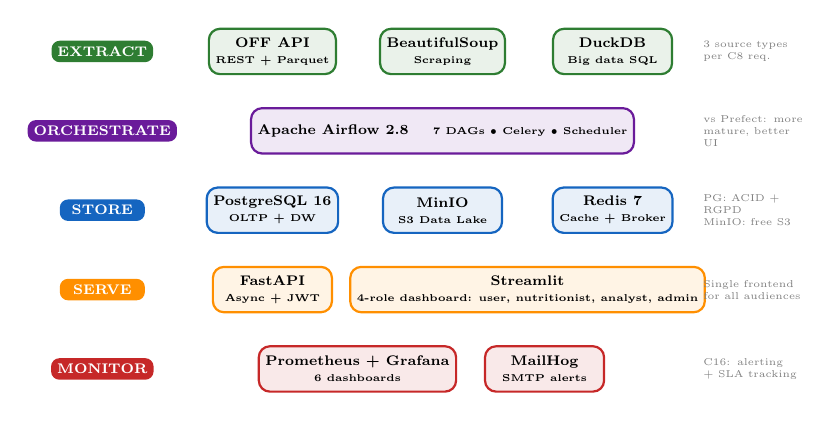
\begin{tikzpicture}[scale=0.72, transform shape,
  tool/.style={rounded corners=4pt, minimum width=2.1cm, minimum height=0.8cm,
               draw, thick, font=\scriptsize\bfseries, align=center},
  why/.style={font=\tiny, text=gray, align=left, text width=1.8cm},
  lbl/.style={font=\scriptsize\bfseries, rounded corners=3pt, inner sep=3pt,
              minimum width=1.5cm, text=white},
]
  \node[lbl, fill=ntgreen]  at (-2, 0)   {EXTRACT};
  \node[lbl, fill=ntpurple] at (-2,-1.4) {ORCHESTRATE};
  \node[lbl, fill=ntblue]   at (-2,-2.8) {STORE};
  \node[lbl, fill=ntaccent] at (-2,-4.2) {SERVE};
  \node[lbl, fill=ntred]    at (-2,-5.6) {MONITOR};

  \node[tool, fill=ntgreen!10, draw=ntgreen] at (1,0) {OFF API\\{\tiny REST + Parquet}};
  \node[tool, fill=ntgreen!10, draw=ntgreen] at (4,0) {BeautifulSoup\\{\tiny Scraping}};
  \node[tool, fill=ntgreen!10, draw=ntgreen] at (7,0) {DuckDB\\{\tiny Big data SQL}};
  \node[why] at (9.5,0) {3 source types\\per C8 req.};

  \node[tool, fill=ntpurple!10, draw=ntpurple, minimum width=6cm] at (4,-1.4)
    {Apache Airflow 2.8 \quad {\tiny 7 DAGs $\bullet$ Celery $\bullet$ Scheduler}};
  \node[why] at (9.5,-1.4) {vs Prefect: more\\mature, better UI};

  \node[tool, fill=ntblue!10, draw=ntblue] at (1,-2.8) {PostgreSQL 16\\{\tiny OLTP + DW}};
  \node[tool, fill=ntblue!10, draw=ntblue] at (4,-2.8) {MinIO\\{\tiny S3 Data Lake}};
  \node[tool, fill=ntblue!10, draw=ntblue] at (7,-2.8) {Redis 7\\{\tiny Cache + Broker}};
  \node[why] at (9.5,-2.8) {PG: ACID + RGPD\\MinIO: free S3};

  \node[tool, fill=ntaccent!10, draw=ntaccent] at (1,-4.2) {FastAPI\\{\tiny Async + JWT}};
  \node[tool, fill=ntaccent!10, draw=ntaccent, minimum width=4.5cm] at (5.5,-4.2) {Streamlit\\{\tiny 4-role dashboard: user, nutritionist, analyst, admin}};
  \node[why] at (9.5,-4.2) {Single frontend\\for all audiences};

  \node[tool, fill=ntred!10, draw=ntred] at (2.5,-5.6) {Prometheus + Grafana\\{\tiny 6 dashboards}};
  \node[tool, fill=ntred!10, draw=ntred] at (5.8,-5.6) {MailHog\\{\tiny SMTP alerts}};
  \node[why] at (9.5,-5.6) {C16: alerting\\+ SLA tracking};
\end{tikzpicture}
\end{center}
\end{frame}

% ======================= SLIDE 8: TECH DECISIONS ==============
\begin{frame}{Key Technical Decisions \competency{C3}}
\begin{center}
\begin{tikzpicture}[scale=0.92, transform shape,
  chosen/.style={rounded corners=5pt, minimum width=2.8cm, minimum height=2cm,
                 fill=ntgreen!8, draw=ntgreen, thick, align=center, font=\scriptsize},
  rejected/.style={rounded corners=5pt, minimum width=2.8cm, minimum height=1.5cm,
                   fill=gray!5, draw=gray!40, align=center, font=\scriptsize, text=gray},
  vs/.style={font=\tiny\bfseries, fill=vsbox, rounded corners=3pt, inner sep=2pt},
]
  \node[chosen] at (0,1.5) {\faDatabase\\[2pt]\textbf{PostgreSQL 16}\\{\tiny ACID + RGPD delete}\\{\tiny OLTP + OLAP}};
  \node[rejected] at (0,-0.8) {MongoDB\\{\tiny No ACID, hard RGPD}};
  \node[vs] at (0,0.25) {vs};

  \node[chosen] at (3.8,1.5) {\faCogs\\[2pt]\textbf{Airflow 2.8}\\{\tiny DAG UI, mature}\\{\tiny Celery for scale}};
  \node[rejected] at (3.8,-0.8) {Prefect\\{\tiny Newer, less proven}};
  \node[vs] at (3.8,0.25) {vs};

  \node[chosen] at (7.6,1.5) {\faCloud\\[2pt]\textbf{MinIO (S3)}\\{\tiny Free, self-hosted}\\{\tiny S3-compatible}};
  \node[rejected] at (7.6,-0.8) {AWS S3\\{\tiny Cloud cost, lock-in}};
  \node[vs] at (7.6,0.25) {vs};

  \node[chosen] at (11.4,1.5) {\faDesktop\\[2pt]\textbf{Streamlit}\\{\tiny 4-role RBAC}\\{\tiny Single frontend}};
  \node[rejected] at (11.4,-0.8) {Superset\\{\tiny Extra service overhead}};
  \node[vs] at (11.4,0.25) {vs};

  \node[font=\tiny, ntgreen] at (0,2.8) {\faCheckCircle\ Selected};
  \node[font=\tiny, ntgreen] at (3.8,2.8) {\faCheckCircle\ Selected};
  \node[font=\tiny, ntgreen] at (7.6,2.8) {\faCheckCircle\ Selected};
  \node[font=\tiny, ntgreen] at (11.4,2.8) {\faCheckCircle\ Selected};
\end{tikzpicture}
\end{center}
\end{frame}

% ======================= SLIDE 9: THREE SCHEMAS ===============
\begin{frame}{PostgreSQL --- Three Zones, One Database}
\begin{center}
\begin{tikzpicture}[scale=0.88, transform shape,
  zone/.style={rounded corners=8pt, minimum width=3.8cm, minimum height=3cm,
               draw, very thick, align=center, font=\scriptsize, inner sep=6pt},
]
  \node[zone, fill=ntaccent!8, draw=ntaccent] (app) at (0,0) {
    \faServer\ \textbf{\normalsize app schema}\\[6pt]
    {\small The Live Application}\\[4pt]
    products, users, meals\\
    brands, categories\\[4pt]
    {\tiny\color{ntaccent} Used by: FastAPI + Streamlit}
  };
  \node[zone, fill=ntblue!8, draw=ntblue] (dw) at (5.5,0) {
    \faStar\ \textbf{\normalsize dw schema}\\[6pt]
    {\small The Warehouse}\\[4pt]
    7 dims + 2 facts\\
    6 datamart views\\[4pt]
    {\tiny\color{ntblue} Used by: Streamlit Analyst}
  };
  \node[zone, fill=ntpurple!8, draw=ntpurple] (lake) at (11,0) {
    \faCloud\ \textbf{\normalsize MinIO}\\[6pt]
    {\small The Data Lake}\\[4pt]
    bronze / silver / gold\\
    Parquet files only\\[4pt]
    {\tiny\color{ntpurple} Used by: Data scientists}
  };

  \draw[-{Stealth}, very thick, gray!40] (app) -- node[above, font=\tiny\bfseries] {ETL} (dw);
  \draw[-{Stealth}, very thick, gray!40] (app.east) ++(0.3,0) |- ++(2,-2) -| (lake.south);
  \node[font=\tiny\bfseries, gray] at (8,-2) {ETL (parallel)};
\end{tikzpicture}
\end{center}
\end{frame}

% ======================= SLIDE 10: DW vs LAKE =================
\begin{frame}{Why Both a Warehouse AND a Lake?}
\begin{center}
\begin{tikzpicture}[
  col/.style={rounded corners=6pt, minimum width=5.5cm, minimum height=4cm,
              draw, thick, align=left, font=\scriptsize, inner sep=8pt},
]
  \node[col, fill=ntblue!5, draw=ntblue] (dw) at (-3.5,0) {
    \textbf{\normalsize Data Warehouse (PostgreSQL)}\\[6pt]
    \faCheckCircle\ Product data \textbf{+} User data\\
    \faLock\ ACID transactions\\
    \faTrashAlt\ Row-level RGPD delete\\
    \faUserCheck\ Consent filtering per query\\
    \faTachometerAlt\ $<$100ms dashboard queries\\[4pt]
    {\tiny\color{ntblue}\faArrowRight\ For BI analysts, dashboards}
  };

  \node[col, fill=ntpurple!5, draw=ntpurple] (lake) at (3.5,0) {
    \textbf{\normalsize Data Lake (MinIO)}\\[6pt]
    \faCheckCircle\ Product data \textbf{ONLY}\\
    \faTimesCircle\ \textbf{No user data --- ever}\\
    \faFile*\ Parquet files (immutable)\\
    \faExpand\ Schema flexibility\\
    \faDatabase\ Bulk reads (ML training)\\[4pt]
    {\tiny\color{ntpurple}\faArrowRight\ For data scientists, ML}
  };

  \node[font=\scriptsize\bfseries, ntred, text width=5cm, align=center] at (0,-3.2) {
    \faShieldAlt\ \textbf{RGPD Boundary:} User data never enters the lake.\\
    Parquet files are immutable --- you cannot delete one user's rows.
  };
\end{tikzpicture}
\end{center}
\end{frame}

% =============================================================
\section{E2 --- Architecture (C2, C3, C4, C6)}
% =============================================================

% ======================= SLIDE 13: TOPOGRAPHY =================
\begin{frame}{Data Topography --- 4 Parts \competency{C2}}
\begin{center}
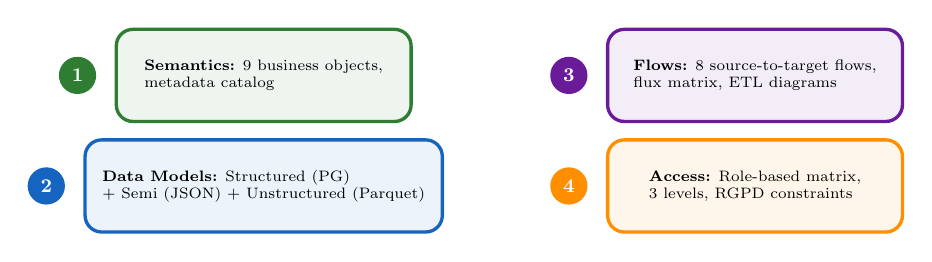
\begin{tikzpicture}[scale=0.78, transform shape,
  part/.style={rounded corners=6pt, minimum width=4.8cm, minimum height=1.5cm,
               draw, very thick, align=left, font=\scriptsize, inner sep=8pt},
  numcirc/.style={circle, text=white, font=\small\bfseries, minimum size=0.6cm},
]
  \node[part, fill=ntgreen!8, draw=ntgreen] (p1) at (-3.2,1.2) {
    \textbf{Semantics:} 9 business objects,\\metadata catalog};
  \node[numcirc, fill=ntgreen, left=0.3cm of p1] {1};

  \node[part, fill=ntblue!8, draw=ntblue] (p2) at (-3.2,-0.6) {
    \textbf{Data Models:} Structured (PG)\\+ Semi (JSON) + Unstructured (Parquet)};
  \node[numcirc, fill=ntblue, left=0.3cm of p2] {2};

  \node[part, fill=ntpurple!8, draw=ntpurple] (p3) at (4.8,1.2) {
    \textbf{Flows:} 8 source-to-target flows,\\flux matrix, ETL diagrams};
  \node[numcirc, fill=ntpurple, left=0.3cm of p3] {3};

  \node[part, fill=ntaccent!8, draw=ntaccent] (p4) at (4.8,-0.6) {
    \textbf{Access:} Role-based matrix,\\3 levels, RGPD constraints};
  \node[numcirc, fill=ntaccent, left=0.3cm of p4] {4};
\end{tikzpicture}
\end{center}
\vspace{0.2cm}
\whycallout{C2 requires mapping ALL data in 4 dimensions --- semantics, models, flows, and access conditions.}
\end{frame}

% ======================= SLIDE 14: ARCHITECTURE ===============
\begin{frame}{System Architecture --- 14 Services \competency{C3}}
\begin{center}
\begin{tikzpicture}[scale=0.62, transform shape,
  svc/.style={rounded corners=4pt, minimum width=1.7cm, minimum height=0.6cm,
              draw, thick, font=\tiny\bfseries, align=center, drop shadow={opacity=0.1}},
]
  \node[svc, fill=ntgreen!15, draw=ntgreen] (s1) at (0,5) {OFF API};
  \node[svc, fill=ntgreen!15, draw=ntgreen] (s2) at (2.5,5) {Parquet};
  \node[svc, fill=ntgreen!15, draw=ntgreen] (s3) at (5,5) {Scraping};
  \node[svc, fill=ntpurple!15, draw=ntpurple, minimum width=5cm] (af) at (2.5,3.2) {Airflow (Web + Sched + Worker)};
  \node[svc, fill=ntblue!15, draw=ntblue] (pg) at (0,1.4) {PostgreSQL\\{\tiny :5432}};
  \node[svc, fill=ntblue!15, draw=ntblue] (mn) at (2.5,1.4) {MinIO\\{\tiny :9000}};
  \node[svc, fill=ntblue!15, draw=ntblue] (rd) at (5,1.4) {Redis\\{\tiny :6379}};
  \node[svc, fill=ntaccent!15, draw=ntaccent] (api) at (0,-0.4) {FastAPI\\{\tiny :8000}};
  \node[svc, fill=ntaccent!15, draw=ntaccent, minimum width=2.5cm] (st) at (3.5,-0.4) {Streamlit\\{\tiny :8501 (4 roles)}};
  \node[svc, fill=ntred!15, draw=ntred] (pr) at (8.5,3.2) {Prometheus};
  \node[svc, fill=ntred!15, draw=ntred] (gf) at (8.5,1.4) {Grafana\\{\tiny :3000}};
  \node[svc, fill=ntred!15, draw=ntred] (mh) at (8.5,-0.4) {MailHog\\{\tiny :8025}};

  \foreach \s in {s1,s2,s3} \draw[-{Stealth}, gray, thick] (\s) -- (af);
  \draw[-{Stealth}, gray, thick] (af) -- (pg);
  \draw[-{Stealth}, gray, thick] (af) -- (mn);
  \draw[-{Stealth}, gray, thick] (pg) -- (api);
  \draw[-{Stealth}, gray, thick] (api) -- (st);
  \draw[-{Stealth}, gray, thick] (rd) -- (api);
  \draw[-{Stealth}, gray, thick] (pr) -- (gf);
  \draw[-{Stealth}, dashed, ntaccent, thick] (af) -- (mh);

  \node[font=\scriptsize] at (0,-1.3) {\faCode\ Devs};
  \node[font=\scriptsize] at (3.5,-1.3) {\faUsers\ All audiences};
\end{tikzpicture}
\end{center}
\end{frame}

% ======================= SLIDE 15: FLUX MATRIX ================
\begin{frame}{Flux Matrix --- 8 Data Flows \competency{C2} \competency{C3}}
\small
\begin{center}
\begin{tabular}{lllll}
  \toprule
  \textbf{Source} & \textbf{Format} & \textbf{Target} & \textbf{Script} & \textbf{Freq.} \\
  \midrule
  OFF API & JSON & /data/raw/api/ & extract\_off\_api.py & Daily \\
  OFF Parquet & Parquet & /data/raw/parquet/ & extract\_off\_parquet.py & Weekly \\
  ANSES/EFSA & HTML & /data/raw/scraping/ & extract\_scraping.py & Monthly \\
  PostgreSQL & SQL & /data/raw/database/ & extract\_from\_db.py & On-demand \\
  DuckDB & Parquet & /data/raw/duckdb/ & extract\_duckdb.py & On-demand \\
  Cleaned data & Parquet & PostgreSQL app & import\_to\_db.py & Daily \\
  App schema & SQL & DW star schema & etl\_load\_warehouse & Daily \\
  Raw files & Mixed & MinIO buckets & etl\_datalake\_ingest & Daily \\
  \bottomrule
\end{tabular}
\end{center}
\end{frame}

% ======================= SLIDE 16: VEILLE =====================
\begin{frame}{Technical Monitoring Newsletter \competency{C4}}
\begin{center}
\begin{tikzpicture}[
  topic/.style={rounded corners=6pt, minimum width=3.6cm, minimum height=2.4cm,
                draw, thick, align=center, font=\scriptsize, inner sep=6pt},
]
  \node[topic, fill=ntaccent!8, draw=ntaccent] at (0,0) {
    \faDesktop\ \textbf{Streamlit RBAC}\\[3pt]
    {\tiny 4-role dashboard}\\{\tiny Replaced Superset BI}\\[3pt]
    {\tiny\color{ntgreen}\faCheckCircle\ Applied}
  };
  \node[topic, fill=ntblue!8, draw=ntblue] at (4.5,0) {
    \faGavel\ \textbf{GDPR Update}\\[3pt]
    {\tiny EDPB Guidelines 01/2026}\\{\tiny Wellness = sensitive data}\\[3pt]
    {\tiny\color{ntgreen}\faCheckCircle\ Compliant}
  };
  \node[topic, fill=ntpurple!8, draw=ntpurple] at (9,0) {
    \faStream\ \textbf{Airflow 2.8}\\[3pt]
    {\tiny Object storage backend}\\{\tiny Listener hooks}\\[3pt]
    {\tiny\color{ntaccent}\faLightbulb\ Future}
  };
\end{tikzpicture}
\end{center}
\vspace{0.2cm}

\begin{tikzpicture}
  \node[rounded corners=6pt, fill=ntgreen!5, draw=ntgreen!40, inner sep=6pt,
        text width=\linewidth-25pt, font=\small] {
    \faClock\ Weekly (1h/week) \quad
    \faCheckDouble\ Sources verified \quad
    \faFile*\ \texttt{docs/veille\_technologique.md}
  };
\end{tikzpicture}
\end{frame}

% ======================= SLIDE 17: RGPD ======================
\begin{frame}{RGPD Compliance --- How It Works \competency{C3} \competency{C11}}
\begin{center}

\begin{tikzpicture}[scale=0.82, transform shape,
  box/.style={rounded corners=6pt, minimum width=3cm, minimum height=2cm,
              draw, thick, align=center, font=\scriptsize, inner sep=6pt},
]
  \node[box, fill=ntred!8, draw=ntred] at (0,0) {
    \faFile*\ \textbf{Data Registry}\\[4pt]
    {\tiny \texttt{rgpd\_data\_registry} table}\\
    {\tiny Legal basis per field}\\
    {\tiny Retention periods}
  };
  \node[box, fill=ntblue!8, draw=ntblue] at (4,0) {
    \faUserCheck\ \textbf{Consent}\\[4pt]
    {\tiny \texttt{consent\_data\_processing}}\\
    {\tiny \texttt{consent\_date} column}\\
    {\tiny Mandatory at registration}
  };
  \node[box, fill=ntgreen!8, draw=ntgreen] at (8,0) {
    \faTrashAlt\ \textbf{Auto-Cleanup}\\[4pt]
    {\tiny \texttt{rgpd\_cleanup\_expired}}\\
    {\tiny Meals $>$2y deleted}\\
    {\tiny Users past retention}
  };
  \node[box, fill=ntpurple!8, draw=ntpurple] at (12,0) {
    \faLock\ \textbf{Security}\\[4pt]
    {\tiny bcrypt passwords}\\
    {\tiny UUID identification}\\
    {\tiny SHA256 in DW}
  };
\end{tikzpicture}
\end{center}
\vspace{0.1cm}
\whycallout{Personal data stays in PostgreSQL (row-level delete). Public product data goes to both DW and Lake.}
\end{frame}

% =============================================================
\section{E3 --- Project Kickoff (C5, C6, C7)}
% =============================================================

% ======================= SLIDE 18: ROADMAP ====================
\begin{frame}{6-Phase Roadmap \competency{C5}}
\begin{center}
\begin{tikzpicture}[scale=0.9, transform shape,
  phase/.style={rounded corners=5pt, minimum width=1.6cm, minimum height=1.7cm,
                draw=ntgreen, thick, fill=ntgreen!8, font=\tiny\bfseries, align=center},
  week/.style={font=\tiny, ntgreen!70},
]
  \node[phase] (p1) at (0,0) {\faServer\\[2pt]Setup\\{\tiny Docker}\\{\tiny DB init}};
  \node[phase] (p2) at (2.5,0) {\faDownload\\[2pt]Extract\\{\tiny 5 scripts}\\{\tiny 3 DAGs}};
  \node[phase] (p3) at (5,0) {\faFilter\\[2pt]Transform\\{\tiny Clean}\\{\tiny Aggregate}};
  \node[phase] (p4) at (7.5,0) {\faStar\\[2pt]Warehouse\\{\tiny Star schema}\\{\tiny SCD}};
  \node[phase] (p5) at (10,0) {\faCloud\\[2pt]Lake\\{\tiny Medallion}\\{\tiny Catalog}};
  \node[phase] (p6) at (12.5,0) {\faRocket\\[2pt]Deploy\\{\tiny Monitor}\\{\tiny Docs}};
  \node[week] at (0,-1.2) {Wk 1--2};
  \node[week] at (2.5,-1.2) {Wk 3--4};
  \node[week] at (5,-1.2) {Wk 5--6};
  \node[week] at (7.5,-1.2) {Wk 7--8};
  \node[week] at (10,-1.2) {Wk 9--10};
  \node[week] at (12.5,-1.2) {Wk 11--12};
  \foreach \i/\j in {p1/p2,p2/p3,p3/p4,p4/p5,p5/p6}
    \draw[-{Stealth}, very thick, ntgreen!40] (\i)--(\j);
\end{tikzpicture}
\end{center}
\vspace{0.3cm}
\begin{columns}[T]
\begin{column}{0.3\textwidth}\begin{center}
  
\begin{tikzpicture}\node[rounded corners=5pt, fill=ntblue!8, draw=ntblue!40, inner sep=5pt,
    text width=3cm, align=center, font=\scriptsize] {\faCalculator\ \textbf{Fibonacci}\\story points};\end{tikzpicture}
\end{center}\end{column}
\begin{column}{0.3\textwidth}\begin{center}
  
\begin{tikzpicture}\node[rounded corners=5pt, fill=ntpurple!8, draw=ntpurple!40, inner sep=5pt,
    text width=3cm, align=center, font=\scriptsize] {\faSync\ \textbf{Rituals}\\Planning, standup,\\review, retro};\end{tikzpicture}
\end{center}\end{column}
\begin{column}{0.3\textwidth}\begin{center}
  \begin{tikzpicture}\node[rounded corners=5pt, fill=ntaccent!8, draw=ntaccent!40, inner sep=5pt,
    text width=3cm, align=center, font=\scriptsize] {\faUsersCog\ \textbf{5 Roles}\\Data Eng, Platform,\\CI/CD, Auditor, Review};\end{tikzpicture}
\end{center}\end{column}
\end{columns}
\end{frame}

% ======================= SLIDE 19: SUPERVISION ================
\begin{frame}{Tracking Indicators \competency{C6}}
\begin{center}

\begin{tikzpicture}[scale=0.82, transform shape,
  metric/.style={rounded corners=6pt, minimum width=3.3cm, minimum height=1.8cm,
                 draw=ntgreen, thick, fill=ntgreen!8, align=center, font=\scriptsize},
]
  \node[metric] at (0,0) {\faChartLine\\[3pt]\textbf{DAG Success Rate}\\{\tiny Pass/fail per run}};
  \node[metric] at (4.2,0) {\faDatabase\\[3pt]\textbf{Activity Log}\\{\tiny 22 entries, 14 days}};
  \node[metric] at (8.4,0) {\faTachometerAlt\\[3pt]\textbf{Completeness \%}\\{\tiny Per dataset}};
  \node[metric] at (12.6,0) {\faClock\\[3pt]\textbf{ETL Duration}\\{\tiny Trend over time}};
\end{tikzpicture}
\end{center}
\vspace{0.2cm}
\begin{center}

\begin{tikzpicture}
  \node[rounded corners=6pt, fill=ntblue!5, draw=ntblue!40, inner sep=6pt,
        text width=0.92\linewidth, font=\small, align=center] {
    \textbf{Tools:}\; Airflow UI $\bullet$ Grafana SLA Dashboard $\bullet$ Git history
  };
\end{tikzpicture}
\end{center}
\end{frame}

% ======================= SLIDE 20: COMMUNICATION ==============
\begin{frame}{Multi-Audience Communication \competency{C7}}
\begin{center}
\begin{tikzpicture}[
  aud/.style={rounded corners=6pt, minimum width=3.5cm, minimum height=2.5cm,
              draw, thick, align=center, font=\scriptsize, inner sep=6pt},
]
  \node[aud, fill=ntgreen!8, draw=ntgreen] at (0,0) {
    \faCode\ \textbf{Developers}\\[6pt]
    Swagger / ReDoc\\Grafana dashboards\\Git + MkDocs
  };
  \node[aud, fill=ntblue!8, draw=ntblue] at (5,0) {
    \faChartPie\ \textbf{Analysts}\\[6pt]
    Streamlit analytics\\Product insights\\Data catalog
  };
  \node[aud, fill=ntaccent!8, draw=ntaccent] at (10,0) {
    \faUsers\ \textbf{End Users}\\[6pt]
    Streamlit app\\Product search\\Meal tracking
  };
\end{tikzpicture}
\end{center}
\vspace{0.2cm}
\whycallout{Right tool for right audience. Technical stakeholders get Swagger; analysts get Streamlit Product Analytics + Data Catalog; users get Streamlit meal tracking.}
\end{frame}

% =============================================================
\section{E4 --- Data Collection \& API (C8--C12)}
% =============================================================

% ======================= SLIDE 21: 5 SOURCES ==================
\begin{frame}{5 Extraction Sources \competency{C8}}
\begin{center}
\begin{tikzpicture}[scale=0.82, transform shape,
  src/.style={rounded corners=5pt, minimum width=2.3cm, minimum height=1.6cm,
              draw, very thick, font=\scriptsize, align=center},
]
  \node[src, fill=ntgreen!10, draw=ntgreen] (a) at (0,0) {\faGlobe\\[2pt]\textbf{REST API}\\{\tiny 1k+ products/day}};
  \node[src, fill=ntblue!10, draw=ntblue] (b) at (3.2,0) {\faFile\\[2pt]\textbf{Data File}\\{\tiny 798k Parquet}};
  \node[src, fill=ntpurple!10, draw=ntpurple] (c) at (6.4,0) {\faCode\\[2pt]\textbf{Scraping}\\{\tiny ANSES/EFSA}};
  \node[src, fill=ntaccent!10, draw=ntaccent] (d) at (9.6,0) {\faServer\\[2pt]\textbf{Database}\\{\tiny PostgreSQL}};
  \node[src, fill=ntred!10, draw=ntred] (e) at (12.8,0) {\faCubes\\[2pt]\textbf{Big Data}\\{\tiny DuckDB 3M+}};

  \node[rounded corners=8pt, fill=ntgreen!5, draw=ntgreen, very thick,
        minimum width=4cm, minimum height=0.8cm, font=\small\bfseries]
        (out) at (6.4,-2.5) {\faFilter\ aggregate\_clean.py};

  \foreach \s in {a,b,c,d,e}
    \draw[-{Stealth}, thick, gray!60] (\s) -- (out);
\end{tikzpicture}
\end{center}
\vspace{0.1cm}
\whycallout{C8 requires 5 source types: REST API, data file, web scraping, database, big data system.}
\end{frame}

% ======================= SLIDE 22: REST API DETAIL ============
\begin{frame}{Source 1: Open Food Facts REST API \competency{C8}}
\begin{columns}[T]
\begin{column}{0.5\textwidth}
\begin{tikzpicture}[
  stepnode/.style={rounded corners=4pt, minimum width=4.5cm, minimum height=0.5cm,
               fill=ntgreen!8, draw=ntgreen!40, font=\scriptsize, align=left, inner xsep=6pt},
]
  \node[font=\small\bfseries, ntgreen] at (0,2.5) {extract\_off\_api.py};
  \node[stepnode] at (0,1.8) {\faCog\ Configure 5 food categories};
  \node[stepnode] at (0,1.1) {\faGlobe\ Paginated GET requests};
  \node[stepnode] at (0,0.4) {\faClock\ Rate limiting (0.6s delay)};
  \node[stepnode] at (0,-0.3) {\faShieldAlt\ User-Agent header};
  \node[stepnode] at (0,-1.0) {\faExclamationTriangle\ Try/except per page};
  \node[stepnode] at (0,-1.7) {\faSave\ Save JSON to /data/raw/api/};
\end{tikzpicture}
\end{column}
\begin{column}{0.45\textwidth}
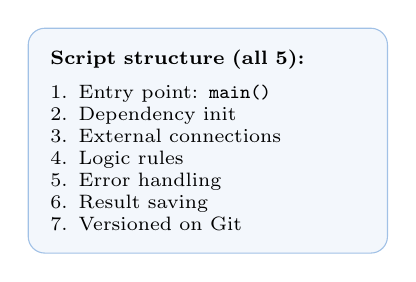
\begin{tikzpicture}
  \node[rounded corners=6pt, fill=ntblue!5, draw=ntblue!40, inner sep=8pt,
        text width=4cm, font=\scriptsize] {
    \textbf{Script structure (all 5):}\\[4pt]
    1. Entry point: \texttt{main()}\\
    2. Dependency init\\
    3. External connections\\
    4. Logic rules\\
    5. Error handling\\
    6. Result saving\\
    7. Versioned on Git
  };
\end{tikzpicture}
\end{column}
\end{columns}
\end{frame}

% ======================= SLIDE 23: SCRAPING + DUCKDB ==========
\begin{frame}{Source 3: Web Scraping \& Source 5: DuckDB \competency{C8}}
\begin{columns}[T]
\begin{column}{0.48\textwidth}
  \begin{center}
  {\small\textbf{\faCode\ Web Scraping}}\\[0.3cm]
  \begin{tikzpicture}
    \node[rounded corners=6pt, fill=ntpurple!5, draw=ntpurple, thick, inner sep=8pt,
          text width=4.2cm, font=\scriptsize] {
      \textbf{extract\_scraping.py}\\[4pt]
      \faGlobe\ Targets: ANSES + EFSA\\
      \faFilter\ BeautifulSoup parsing\\
      \faAppleAlt\ Nutritional guidelines\\
      \faSyncAlt\ Fallback RDA values\\
      \faSave\ JSON output\\[4pt]
      {\tiny Frequency: Monthly}
    };
  \end{tikzpicture}
  \end{center}
\end{column}
\begin{column}{0.48\textwidth}
  \begin{center}
  {\small\textbf{\faCubes\ DuckDB Big Data}}\\[0.3cm]
  \begin{tikzpicture}
    \node[rounded corners=6pt, fill=ntred!5, draw=ntred, thick, inner sep=8pt,
          text width=4.2cm, font=\scriptsize] {
      \textbf{extract\_duckdb.py}\\[4pt]
      \faDatabase\ SQL on Parquet files\\
      \faExpand\ 3M+ rows, no DB needed\\
      \faChartBar\ Analytical aggregations\\
      \faTachometerAlt\ Columnar = fast scans\\
      \faSave\ Parquet output\\[4pt]
      {\tiny SQL on Parquet files}
    };
  \end{tikzpicture}
  \end{center}
\end{column}
\end{columns}
\end{frame}

% ======================= SLIDE 24: CLEANING ===================
\begin{frame}{Cleaning Pipeline \competency{C10}}
\begin{center}
\begin{tikzpicture}[
  sn/.style={rounded corners=4pt, minimum width=10.5cm, minimum height=0.55cm,
               font=\scriptsize, align=left, inner xsep=8pt},
]
  \node[font=\small\bfseries] at (0,3.5) {aggregate\_clean.py --- 7 cleaning steps};
  \node[font=\tiny, ntpurple] at (0,3.0) {\textbf{Engine:} PySpark 3.5 (distributed-capable)};

  \node[sn, fill=ntred!8, draw=ntred]       at (0,2.5) {\faColumns\ \textbf{1.} Standardize 30+ column names across all sources};
  \node[sn, fill=ntaccent!8, draw=ntaccent]  at (0,1.7) {\faBarcode\ \textbf{2.} Validate barcodes (strip non-numeric, check 8--14 digits)};
  \node[sn, fill=ntaccent!8, draw=ntaccent]  at (0,0.9) {\faTrash\ \textbf{3.} Remove rows with null product names};
  \node[sn, fill=ntpurple!8, draw=ntpurple]  at (0,0.1) {\faRuler\ \textbf{4.} Cap nutritional values at physiological max per 100g};
  \node[sn, fill=ntblue!8, draw=ntblue]      at (0,-0.7) {\faFont\ \textbf{5.} Normalize Nutri-Score to uppercase A--E};
  \node[sn, fill=ntgreen!8, draw=ntgreen]    at (0,-1.5) {\faCopy\ \textbf{6.} Deduplicate by barcode (keep most complete)};
  \node[sn, fill=ntgreen!8, draw=ntgreen]    at (0,-2.3) {\faClipboardCheck\ \textbf{7.} Generate cleaning\_report.json};

  \draw[-{Stealth}, very thick, gray!30] (5.8,2.7) -- (5.8,-2.5);
\end{tikzpicture}
\end{center}
\vspace{0.1cm}
{\scriptsize\faCheckDouble\ \textbf{6 formal validation checks} logged to \texttt{staging.data\_quality\_checks} table (nulls, ranges, duplicates, formats, referential integrity, completeness).}
\end{frame}

% ======================= SLIDE 25: SQL =======================
\begin{frame}{7 Optimized SQL Queries \competency{C9}}
\small
\begin{center}
\begin{tabular}{clll}
  \toprule
  \textbf{\#} & \textbf{Query} & \textbf{Technique} & \textbf{Optimization} \\
  \midrule
  1 & Full-text product search & GIN index, \texttt{ts\_rank} & Index scan \\
  2 & User nutrition summary & \texttt{ROW\_NUMBER() OVER} & Window partition \\
  3 & Product market analysis & CTE + aggregation & CTE avoids re-scan \\
  4 & Brand comparison & Analytical functions & Composite index \\
  5 & Temporal trends & \texttt{LAG()}, moving avg & Partial index \\
  6 & Category aggregation & \texttt{GROUP BY + HAVING} & Aggregate pushdown \\
  7 & Complex joins & Materialized + joins & Pre-computed \\
  \bottomrule
\end{tabular}
\end{center}
\vspace{0.2cm}
{\small All queries documented with \texttt{EXPLAIN ANALYZE} and optimization rationale.}
\end{frame}

% ======================= SLIDE 26: DATABASE ===================
\begin{frame}{RGPD-Compliant Database \competency{C11}}
\begin{center}
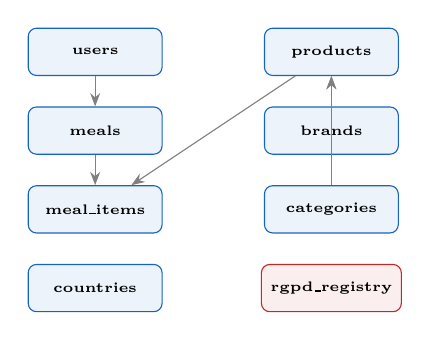
\begin{tikzpicture}[
  tbl/.style={rounded corners=3pt, minimum width=1.7cm, minimum height=0.6cm,
              draw=ntblue, fill=ntblue!8, font=\tiny\bfseries},
]
  \node[tbl] (u) at (0,2.5) {users};
  \node[tbl] (p) at (3,2.5) {products};
  \node[tbl] (b) at (3,1.5) {brands};
  \node[tbl] (c) at (3,0.5) {categories};
  \node[tbl] (m) at (0,1.5) {meals};
  \node[tbl] (mi) at (0,0.5) {meal\_items};
  \node[tbl] (cc) at (0,-0.5) {countries};
  \node[tbl, draw=ntred, fill=ntred!8] (r) at (3,-0.5) {rgpd\_registry};
  \draw[-{Stealth}, gray, thin] (u)--(m);
  \draw[-{Stealth}, gray, thin] (m)--(mi);
  \draw[-{Stealth}, gray, thin] (p)--(mi);
  \draw[-{Stealth}, gray, thin] (b)--(p);
  \draw[-{Stealth}, gray, thin] (c)--(p);
\end{tikzpicture}
\quad
\begin{tikzpicture}
  \node[rounded corners=6pt, fill=ntgreen!5, draw=ntgreen, thick, inner sep=8pt,
        text width=5cm, font=\scriptsize, align=left] {
    \textbf{MERISE:} MCD $\to$ MLD $\to$ MPD\\[4pt]
    \faShieldAlt\ \texttt{rgpd\_data\_registry} table\\
    \faUserCheck\ Consent columns\\
    \faTrashAlt\ \texttt{rgpd\_cleanup\_expired\_data()}\\
    \faLock\ bcrypt password hashing\\
    \faFingerprint\ UUID-based identification\\[4pt]
    \textbf{8 tables}, full referential integrity
  };
\end{tikzpicture}
\end{center}
\end{frame}

% ======================= SLIDE 27: API =======================
\begin{frame}{FastAPI REST API \competency{C12}}
\begin{columns}[T]
\begin{column}{0.5\textwidth}
  \begin{center}
  \begin{tikzpicture}[
    ep/.style={rounded corners=3pt, minimum width=4.3cm, minimum height=0.42cm,
               draw=ntaccent!60, fill=ntaccent!5, font=\tiny, align=left, inner xsep=5pt},
  ]
    \node[font=\small\bfseries, ntaccent] at (0,2.2) {Endpoints};
    \node[ep] at (0,1.65) {\faLock\ POST /auth/register};
    \node[ep] at (0,1.1) {\faLock\ POST /auth/login};
    \node[ep] at (0,0.55) {\faSearch\ GET /products/?q=\&nutriscore=};
    \node[ep] at (0,0) {\faBarcode\ GET /products/\{barcode\}};
    \node[ep] at (0,-0.55) {\faHeart\ GET /products/\{barcode\}/alternatives};
    \node[ep] at (0,-1.1) {\faUtensils\ POST /meals};
    \node[ep] at (0,-1.65) {\faChartLine\ GET /meals/daily-summary};
    \node[ep] at (0,-2.2) {\faChartArea\ GET /meals/weekly-trends};
  \end{tikzpicture}
  \end{center}
\end{column}
\begin{column}{0.45\textwidth}
  \begin{center}
  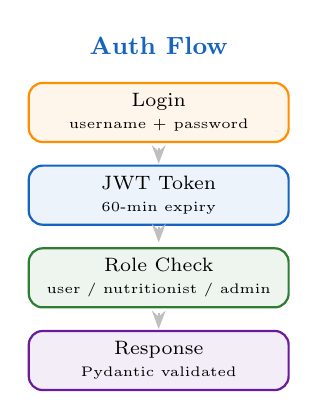
\begin{tikzpicture}[
    stepnode/.style={rounded corners=5pt, minimum width=3.3cm, minimum height=0.75cm,
                 draw, thick, align=center, font=\scriptsize},
  ]
    \node[font=\small\bfseries, ntblue] at (0,2.0) {Auth Flow};
    \node[stepnode, fill=ntaccent!8, draw=ntaccent] at (0,1.15) {Login\\{\tiny username + password}};
    \node[stepnode, fill=ntblue!8, draw=ntblue] at (0,0.1) {JWT Token\\{\tiny 60-min expiry}};
    \node[stepnode, fill=ntgreen!8, draw=ntgreen] at (0,-0.95) {Role Check\\{\tiny user / nutritionist / admin}};
    \node[stepnode, fill=ntpurple!8, draw=ntpurple] at (0,-2.0) {Response\\{\tiny Pydantic validated}};
    \draw[-{Stealth}, thick, gray!50] (0,0.7)--(0,0.5);
    \draw[-{Stealth}, thick, gray!50] (0,-0.3)--(0,-0.5);
    \draw[-{Stealth}, thick, gray!50] (0,-1.4)--(0,-1.6);
  \end{tikzpicture}
  \end{center}
\end{column}
\end{columns}
\vspace{-0.2cm}
\democallout{Show Swagger UI at localhost:8000/docs}
\end{frame}

% ======================= SLIDE 28: STREAMLIT ==================
\begin{frame}{Streamlit --- 4 Roles, 1 Frontend \competency{C7} \competency{C12} \competency{C20}}
\begin{center}
\begin{tikzpicture}[
  rolecard/.style={rounded corners=6pt, minimum width=2.8cm, minimum height=3.5cm,
                   draw, thick, align=left, font=\scriptsize, inner sep=6pt},
]
  \node[rolecard, fill=ntaccent!8, draw=ntaccent] at (0,0) {
    \faUser\ \textbf{User}\\[4pt]
    \faSearch\ Product search\\
    \faUtensils\ Meal logger\\
    \faChartPie\ Daily dashboard\\
    \faChartLine\ Weekly trends\\
    \faBalanceScale\ Comparison\\
    \faHeart\ Alternatives
  };
  \node[rolecard, fill=ntblue!8, draw=ntblue] at (3.5,0) {
    \faUserMd\ \textbf{Nutritionist}\\[4pt]
    {\tiny All user pages +}\\
    \faUsers\ User analytics\\
    \faChartBar\ Caloric analysis\\
    \faTrashAlt\ User management\\
    \faFilter\ Goal/activity filters
  };
  \node[rolecard, fill=ntpurple!8, draw=ntpurple] at (7,0) {
    \faChartPie\ \textbf{Analyst}\\[4pt]
    {\tiny All user pages +}\\
    \faStar\ Product analytics\\
    \faDatabase\ Data catalog\\
    \faSearch\ Brand rankings\\
    \faChartBar\ Nutri-Score stats
  };
  \node[rolecard, fill=ntred!8, draw=ntred] at (10.5,0) {
    \faUserShield\ \textbf{Admin}\\[4pt]
    {\tiny All pages +}\\
    \faUsers\ Nutritionist view\\
    \faStar\ Analyst view\\
    \faDatabase\ Data catalog\\
    \faTrashAlt\ Full management
  };
\end{tikzpicture}
\end{center}
\vspace{0.1cm}
\whycallout{Single Streamlit app replaces Superset. JWT role in token controls navigation and API access. Defense-in-depth: UI hides pages + API rejects unauthorized calls.}
\democallout{Show role switching: user $\to$ nutritionist $\to$ analyst $\to$ admin}
\end{frame}

% =============================================================
\section{E5 --- Data Warehouse (C13--C15)}
% =============================================================

% ======================= SLIDE 29: STAR SCHEMA ================
\begin{frame}{Star Schema \competency{C13}}
\begin{center}
\begin{tikzpicture}[scale=0.75, transform shape,
  dim/.style={rounded corners=4pt, minimum width=1.8cm, minimum height=0.7cm,
              draw=ntblue, very thick, fill=ntblue!10, font=\tiny\bfseries, align=center},
  fact/.style={rounded corners=4pt, minimum width=2.5cm, minimum height=1cm,
               draw=ntaccent, very thick, fill=ntaccent!15, font=\small\bfseries, align=center,
               drop shadow={opacity=0.15}},
]
  \node[fact] (f1) at (-3,0) {fact\_daily\\nutrition};
  \node[fact] (f2) at (8,0) {fact\_product\\market};
  \node[dim] (d3) at (2.5,0) {\faBox\ dim\_product};
  \node[dim] (d1) at (2.5,2.5) {\faClock\ dim\_time};
  \node[dim] (d2) at (-3,2.5) {\faUser\ dim\_user};
  \node[dim] (d7) at (-6,-2) {\faAppleAlt\ dim\_nutriscore};
  \node[dim] (d4) at (5,-2.5) {\faTags\ dim\_brand};
  \node[dim] (d5) at (8,-2.5) {\faThList\ dim\_category};
  \node[dim] (d6) at (11,-2) {\faGlobe\ dim\_country};
  \draw[very thick, ntblue!50] (d2)--(f1);
  \draw[very thick, ntblue!50] (d7)--(f1);
  \draw[very thick, ntblue!50] (d3)--(f1);
  \draw[very thick, ntblue!50] (d3)--(f2);
  \draw[very thick, ntblue!50] (d1)--(f1);
  \draw[very thick, ntblue!50] (d1)--(f2);
  \draw[very thick, ntblue!50] (d4)--(f2);
  \draw[very thick, ntblue!50] (d5)--(f2);
  \draw[very thick, ntblue!50] (d6)--(f2);
  \node[font=\tiny\bfseries, ntpurple, fill=white, inner sep=2pt] at (2.5,-0.8) {shared};
  \node[rounded corners=5pt, fill=ntgreen!5, draw=ntgreen!40, inner sep=5pt, font=\scriptsize]
    at (2.5,-4) {\textbf{7 dims} + \textbf{2 facts} + \textbf{6 datamart views}
    \;\;$\bullet$\;\; Bottom-up (Kimball)};
\end{tikzpicture}
\end{center}
\end{frame}

% ======================= SLIDE 30: DATAMARTS ==================
\begin{frame}{6 Datamart Views \competency{C13} \competency{C14}}
\small
\begin{center}
\begin{tabular}{lll}
  \toprule
  \textbf{Datamart View} & \textbf{Purpose} & \textbf{Audience} \\
  \midrule
  dm\_user\_daily\_nutrition & Daily calorie \& macro tracking & Nutritionists \\
  dm\_product\_market\_by\_category & Product availability by category & Market analysts \\
  dm\_brand\_quality\_ranking & Brand ranking by Nutri-Score & Quality team \\
  dm\_nutriscore\_distribution & Nutri-Score distribution (A--E) & Public health \\
  dm\_nutrition\_trends & Weekly/monthly nutrition trends & Data scientists \\
  dm\_dw\_health & DW operational health metrics & DW admins \\
  \bottomrule
\end{tabular}
\end{center}
\vspace{0.2cm}
\whycallout{Datamarts are pre-built SQL views. The Streamlit Analyst dashboard queries these views via FastAPI for product analytics.}
\end{frame}

% ======================= SLIDE 31: ETL PIPELINE ===============
\begin{frame}{ETL Pipeline --- 7 DAGs \competency{C15}}
\begin{center}
\begin{tikzpicture}[
  dag/.style={rounded corners=3pt, minimum width=2.3cm, minimum height=0.5cm,
              draw, thick, font=\tiny\bfseries, align=center},
  time/.style={font=\tiny, gray},
]
  \node[dag, fill=ntgreen!15, draw=ntgreen] (e1) at (0,0) {extract\_off\_api};
  \node[dag, fill=ntgreen!15, draw=ntgreen] (e2) at (0,-0.7) {extract\_parquet};
  \node[dag, fill=ntgreen!15, draw=ntgreen] (e3) at (0,-1.4) {extract\_scraping};
  \node[time] at (-1.8,-0.7) {02:00};

  \node[dag, fill=ntaccent!15, draw=ntaccent] (c) at (4,-0.7) {aggregate\_clean};
  \node[time] at (4,-1.4) {04:00};

  \node[dag, fill=ntblue!15, draw=ntblue] (dw) at (8,-0.2) {load\_warehouse};
  \node[dag, fill=ntpurple!15, draw=ntpurple] (dl) at (8,-1.2) {datalake\_ingest};
  \node[time] at (9.8,-0.7) {05:00};

  \node[dag, fill=ntred!15, draw=ntred] (bk) at (0,-2.8) {backup\_maint.};
  \node[time] at (-1.8,-2.8) {06:00};

  \draw[-{Stealth}, gray, thick] (e1)--(c);
  \draw[-{Stealth}, gray, thick] (e2)--(c);
  \draw[-{Stealth}, gray, thick] (e3)--(c);
  \draw[-{Stealth}, gray, thick] (c)--(dw);
  \draw[-{Stealth}, gray, thick] (c)--(dl);

  \node[font=\tiny\bfseries, ntpurple, fill=white, inner sep=1pt] at (6,-0.3) {parallel};

  % Cross-DAG sensor note
  \node[rounded corners=4pt, fill=whybox, draw=ntblue!40, inner sep=5pt,
        font=\scriptsize, text width=5cm] at (8,-3) {
    \faLink\ \texttt{ExternalTaskSensor} ensures\\
    DW and Lake wait for cleaning to finish
  };
\end{tikzpicture}
\end{center}
\democallout{Show Airflow UI at localhost:8080}
\end{frame}

% ======================= SLIDE 32: SCD ========================
\begin{frame}{SCD --- Slowly Changing Dimensions \competency{C17}}
\begin{center}
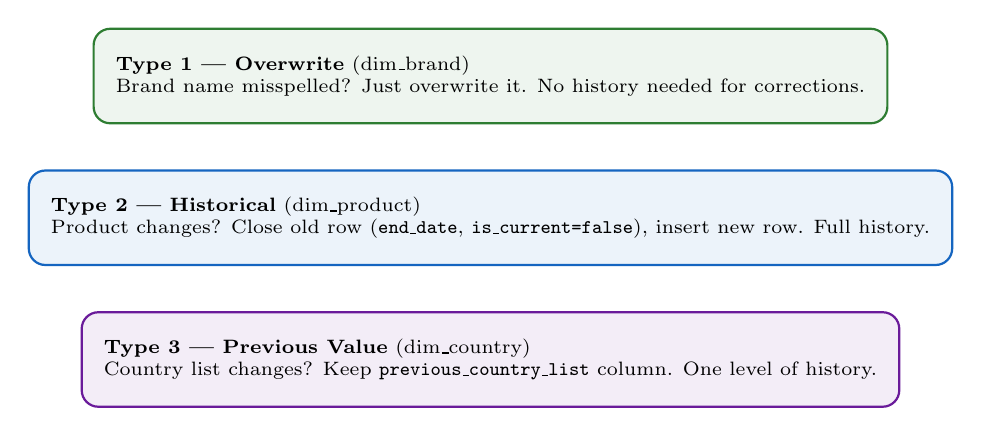
\begin{tikzpicture}[
  scd/.style={rounded corners=6pt, minimum width=10cm, minimum height=1.2cm,
              draw, thick, align=left, font=\scriptsize, inner sep=8pt},
]
  \node[scd, fill=ntgreen!8, draw=ntgreen] at (0,1.8) {
    \textbf{Type 1 --- Overwrite} (dim\_brand)\\
    Brand name misspelled? Just overwrite it. No history needed for corrections.
  };
  \node[scd, fill=ntblue!8, draw=ntblue] at (0,0) {
    \textbf{Type 2 --- Historical} (dim\_product)\\
    Product changes? Close old row (\texttt{end\_date}, \texttt{is\_current=false}), insert new row. Full history.
  };
  \node[scd, fill=ntpurple!8, draw=ntpurple] at (0,-1.8) {
    \textbf{Type 3 --- Previous Value} (dim\_country)\\
    Country list changes? Keep \texttt{previous\_country\_list} column. One level of history.
  };
\end{tikzpicture}
\end{center}
\vspace{0.1cm}
\whycallout{Change detection uses \texttt{IS DISTINCT FROM} in the ETL. All 3 types are integrated into the warehouse loading DAG.}
\end{frame}

% =============================================================
\section{E6 --- DW Maintenance (C16, C17)}
% =============================================================

% ======================= SLIDE 33: ALERT FLOW =================
\begin{frame}{Alert System --- How It Works \competency{C16}}
\begin{center}
\begin{tikzpicture}[scale=0.82, transform shape,
  stepnode/.style={rounded corners=5pt, minimum width=1.8cm, minimum height=1.1cm,
               draw, very thick, align=center, font=\scriptsize},
]
  \node[stepnode, fill=ntred!10, draw=ntred] (fail) at (0,0) {\faExclamationTriangle\\DAG Fails};
  \node[stepnode, fill=ntaccent!10, draw=ntaccent] (plugin) at (3.5,0) {\faCogs\\alerting.py\\callback};
  \node[stepnode, fill=ntblue!10, draw=ntblue] (log) at (7,0.8) {\faDatabase\\activity\_log};
  \node[stepnode, fill=ntpurple!10, draw=ntpurple] (email) at (7,-0.8) {\faEnvelope\\MailHog};
  \node[stepnode, fill=ntgreen!10, draw=ntgreen] (stats) at (10.5,0.8) {\faChartBar\\StatsD};
  \node[stepnode, fill=ntgreen!10, draw=ntgreen] (graf) at (13.5,0) {\faTachometerAlt\\Grafana};
  \draw[-{Stealth}, very thick, ntred!50] (fail)--(plugin);
  \draw[-{Stealth}, very thick, ntblue!50] (plugin)--(log);
  \draw[-{Stealth}, very thick, ntpurple!50] (plugin)--(email);
  \draw[-{Stealth}, very thick, ntgreen!50] (log)--(stats);
  \draw[-{Stealth}, very thick, ntgreen!50] (stats)--(graf);
  \draw[-{Stealth}, very thick, ntpurple!50] (email.east)--++(0.5,0)|-(graf);
\end{tikzpicture}
\end{center}
\end{frame}

% ======================= SLIDE 34: SLA ========================
\begin{frame}{SLA Dashboard \competency{C16}}
\begin{center}
\begin{tikzpicture}[scale=0.85, transform shape,
  sla/.style={rounded corners=5pt, minimum width=3cm, minimum height=1.5cm,
              draw=ntgreen, thick, fill=ntgreen!8, align=center, font=\scriptsize},
]
  \node[sla] at (0,0) {\faCheckCircle\\[3pt]\textbf{ETL Success}\\$>$ 95\%};
  \node[sla] at (4,0) {\faClock\\[3pt]\textbf{Freshness}\\$<$ 24h};
  \node[sla] at (8,0) {\faHdd\\[3pt]\textbf{Backups}\\100\%};
  \node[sla] at (12,0) {\faTachometerAlt\\[3pt]\textbf{Query Time}\\$<$ 5s};
\end{tikzpicture}
\end{center}
\vspace{0.3cm}
\begin{center}
\begin{tikzpicture}
  \node[rounded corners=4pt, fill=ntaccent!8, draw=ntaccent!40, inner sep=6pt,
        font=\scriptsize, text width=9cm, align=center] {
    \textbf{ITIL Priority Matrix:}\quad
    P1 Critical $<$1h \quad P2 High $<$4h \quad P3 Medium $<$24h \quad P4 Low: next sprint\\
    \textbf{Escalation:} L1 (auto-restart) $\to$ L2 (engineer) $\to$ L3 (architecture review)
  };
\end{tikzpicture}
\end{center}
\democallout{Show Grafana SLA dashboard + MailHog alerts}
\end{frame}

% ======================= SLIDE 35: BACKUPS ====================
\begin{frame}{Backup \& Maintenance Procedures \competency{C16}}
\begin{columns}[T]
\begin{column}{0.48\textwidth}
  \begin{center}
  \begin{tikzpicture}
    \node[rounded corners=6pt, fill=ntblue!5, draw=ntblue, thick, inner sep=8pt,
          text width=4.5cm, font=\scriptsize, align=left] {
      \textbf{\faHdd\ Backup Script}\\[4pt]
      \texttt{backup\_database.py}\\[4pt]
      \faDatabase\ Full + partial modes\\
      \faCloud\ Upload to MinIO /backups\\
      \faTrashAlt\ Auto-cleanup old backups\\
      \faCogs\ Airflow DAG scheduled\\[4pt]
      {\tiny 154 lines, Git-versioned}
    };
  \end{tikzpicture}
  \end{center}
\end{column}
\begin{column}{0.48\textwidth}
  \begin{center}
  \begin{tikzpicture}
    \node[rounded corners=6pt, fill=ntgreen!5, draw=ntgreen, thick, inner sep=8pt,
          text width=4.5cm, font=\scriptsize, align=left] {
      \textbf{\faFile*\ Documented Procedures}\\[4pt]
      \faPlus\ New source integration (6 steps)\\
      \faUserPlus\ New access creation (3 steps)\\
      \faExpand\ Storage expansion\\
      \faLayerGroup\ Add datamart view\\
      \faMicrochip\ Compute capacity scaling\\[4pt]
      {\tiny All in rapport\_final Ch.12}
    };
  \end{tikzpicture}
  \end{center}
\end{column}
\end{columns}
\end{frame}

% =============================================================
\section{E7 --- Data Lake (C18--C21)}
% =============================================================

% ======================= SLIDE 36: MEDALLION ==================
\begin{frame}{Medallion Architecture \competency{C18}}
\begin{center}
\begin{tikzpicture}[
  layer/.style={rounded corners=8pt, minimum width=3.5cm, minimum height=2.2cm,
                draw, very thick, font=\small\bfseries, align=center, drop shadow={opacity=0.15}},
]
  \node[layer, fill=bronze!15, draw=bronze, text=bronze!70!black] (b) at (0,0) {
    \faDatabase\ \textbf{Bronze}\\[4pt]
    {\scriptsize Raw as-is}\\{\scriptsize JSON, Parquet, CSV}\\{\scriptsize 90-day retention}
  };
  \node[layer, fill=silver!15, draw=silver!70, text=gray!70!black] (s) at (5.3,0) {
    \faFilter\ \textbf{Silver}\\[4pt]
    {\scriptsize Cleaned \& validated}\\{\scriptsize Parquet only}\\{\scriptsize Deduplicated}
  };
  \node[layer, fill=gold!15, draw=gold, text=gold!50!black] (g) at (10.6,0) {
    \faStar\ \textbf{Gold}\\[4pt]
    {\scriptsize Analytics-ready}\\{\scriptsize ML features, daily snapshots,}\\{\scriptsize anonymized aggregates}
  };
  \draw[-{Stealth}, very thick, bronze!50] (b) -- node[above, font=\scriptsize\bfseries] {clean} (s);
  \draw[-{Stealth}, very thick, silver!50] (s) -- node[above, font=\scriptsize\bfseries] {aggregate} (g);
\end{tikzpicture}
\end{center}
\vspace{0.3cm}
\begin{center}
\begin{tikzpicture}
  \node[rounded corners=6pt, fill=ntgreen!5, draw=ntgreen!40, inner sep=6pt,
        text width=0.92\linewidth, font=\small, align=center] {
    Addresses: \textbf{Volume} (3M+ products) $\bullet$ \textbf{Variety} (JSON, Parquet, CSV) $\bullet$ \textbf{Velocity} (daily/weekly schedules)
  };
\end{tikzpicture}
\end{center}
\end{frame}

% ======================= SLIDE 37: V/V/V =====================
\begin{frame}{Volume, Variety, Velocity \competency{C18}}
\begin{center}
\begin{tikzpicture}[scale=0.9, transform shape,
  v/.style={rounded corners=8pt, minimum width=3.5cm, minimum height=2.5cm,
            draw, very thick, align=center, font=\scriptsize, inner sep=6pt},
]
  \node[v, fill=ntblue!8, draw=ntblue] at (0,0) {
    \faDatabase\ \textbf{\large Volume}\\[6pt]
    3M+ products\\
    798k+ imported\\
    Parquet columnar\\for fast scans
  };
  \node[v, fill=ntpurple!8, draw=ntpurple] at (5.5,0) {
    \faRandom\ \textbf{\large Variety}\\[6pt]
    JSON (API)\\
    Parquet (bulk)\\
    HTML (scraping)\\
    SQL (database)
  };
  \node[v, fill=ntaccent!8, draw=ntaccent] at (11,0) {
    \faTachometerAlt\ \textbf{\large Velocity}\\[6pt]
    Daily API pulls\\
    Weekly Parquet\\
    Monthly scraping\\
    Scheduled DAGs
  };
\end{tikzpicture}
\end{center}
\end{frame}

% ======================= SLIDE 38: CATALOG COMPARISON =========
\begin{frame}{Catalog Tool Comparison \competency{C18}}
\small
\begin{center}
\begin{tabular}{lccc}
  \toprule
  \textbf{Criteria} & \textbf{Apache Atlas} & \textbf{DataHub} & \textbf{\color{ntgreen}Custom JSON} \\
  \midrule
  Setup complexity & High & Medium & \color{ntgreen}\textbf{Low} \\
  Resource overhead & Heavy (Java) & Moderate & \color{ntgreen}\textbf{Minimal} \\
  MinIO integration & Manual & Plugin & \color{ntgreen}\textbf{Native} \\
  Search capability & Full & Full & Basic (Streamlit) \\
  Lineage tracking & Auto & Auto & Manual (JSON) \\
  Fits project scale & Overkill & Overkill & \color{ntgreen}\textbf{Right-sized} \\
  \bottomrule
\end{tabular}
\end{center}
\vspace{0.3cm}
\whycallout{Custom JSON catalog was chosen because Atlas and DataHub add significant infrastructure for a project at this scale. The Streamlit browser provides search and browse capabilities.}
\end{frame}

% ======================= SLIDE 39: CATALOG ====================
\begin{frame}{Data Catalog Browser \competency{C20}}
\begin{center}
\begin{tikzpicture}[
  feat/.style={rounded corners=4pt, minimum width=5cm, minimum height=0.5cm,
               fill=ntpurple!8, draw=ntpurple!40, font=\scriptsize, align=left, inner xsep=6pt},
]
  \node[font=\normalsize\bfseries, ntpurple] at (0,2.3) {Streamlit Catalog Page};
  \node[feat] at (0,1.7) {\faSearch\ Search datasets by name, format, or source};
  \node[feat] at (0,1.05) {\faLayerGroup\ Browse by layer (bronze / silver / gold tabs)};
  \node[feat] at (0,0.4) {\faTable\ View schema (column names + types)};
  \node[feat] at (0,-0.25) {\faProjectDiagram\ View lineage (where data came from)};
  \node[feat] at (0,-0.9) {\faChartBar\ Quality metrics per dataset};
  \node[feat] at (0,-1.55) {\faShieldAlt\ Governance info + RGPD compliance};
  \node[feat] at (0,-2.2) {\faHdd\ Storage stats (object count, total size)};
\end{tikzpicture}
\end{center}
\democallout{Show Streamlit catalog at localhost:8501/data\_catalog}
\end{frame}

% ======================= SLIDE 40: GOVERNANCE =================
\begin{frame}{Access Governance \competency{C21}}
\begin{center}
\begin{tikzpicture}[
  role/.style={rounded corners=6pt, minimum width=12cm, minimum height=0.65cm,
               draw, thick, align=left, font=\scriptsize, inner xsep=8pt},
]
  \node[font=\normalsize\bfseries] at (0,3) {Group-Based Access --- 4 Roles (not individual)};

  \node[role, fill=ntred!8, draw=ntred] at (0,2) {
    \faUserShield\ \textbf{admin} \hfill
    PostgreSQL: full \;$\bullet$\; MinIO: all buckets \;$\bullet$\; API: all endpoints \;$\bullet$\; Streamlit: all pages};
  \node[role, fill=ntpurple!8, draw=ntpurple] at (0,1) {
    \faChartPie\ \textbf{analyst} \hfill
    PostgreSQL: read products \;$\bullet$\; MinIO: gold \;$\bullet$\; API: /analytics \;$\bullet$\; Streamlit: Product Analytics + Catalog};
  \node[role, fill=ntblue!8, draw=ntblue] at (0,0) {
    \faUserMd\ \textbf{nutritionist} \hfill
    PostgreSQL: read products+meals \;$\bullet$\; MinIO: none \;$\bullet$\; API: /nutritionist \;$\bullet$\; Streamlit: User Dashboard};
  \node[role, fill=ntaccent!8, draw=ntaccent] at (0,-1) {
    \faUser\ \textbf{user} \hfill
    PostgreSQL: own meals only \;$\bullet$\; MinIO: none \;$\bullet$\; API: /meals,/products \;$\bullet$\; Streamlit: 6 pages};
\end{tikzpicture}
\end{center}
\vspace{0.3cm}
\whycallout{Least-privilege principle: each role gets only what it needs. Consistent across all 4 systems. RGPD-compliant.}
\end{frame}

% ======================= SLIDE 41: MONITORING =================
\begin{frame}{Monitoring Stack \competency{C16} \competency{C20}}
\begin{center}
\begin{tikzpicture}[
  box/.style={rounded corners=5pt, minimum width=2.2cm, minimum height=1.5cm,
              draw, thick, align=center, font=\scriptsize},
]
  \node[box, fill=ntred!8, draw=ntred] (sd) at (0,0) {\faPaperPlane\\StatsD\\{\tiny Airflow metrics}};
  \node[box, fill=ntred!8, draw=ntred] (ca) at (3,0) {\faDocker\\cAdvisor\\{\tiny Container stats}};
  \node[box, fill=ntred!8, draw=ntred] (ne) at (6,0) {\faServer\\Node Exp.\\{\tiny Host metrics}};
  \node[box, fill=ntred!8, draw=ntred] (pe) at (9,0) {\faDatabase\\PG Exp.\\{\tiny DB metrics}};

  \node[box, fill=ntaccent!10, draw=ntaccent, minimum width=6cm] (pr) at (4.5,-2) {
    \faChartLine\ \textbf{Prometheus} \quad {\tiny scrapes all 4 exporters}};
  \node[box, fill=ntgreen!10, draw=ntgreen, minimum width=4cm] (gf) at (4.5,-4) {
    \faTachometerAlt\ \textbf{Grafana} \quad {\tiny 6 dashboards}};

  \draw[-{Stealth}, thick, gray] (sd)--(pr);
  \draw[-{Stealth}, thick, gray] (ca)--(pr);
  \draw[-{Stealth}, thick, gray] (ne)--(pr);
  \draw[-{Stealth}, thick, gray] (pe)--(pr);
  \draw[-{Stealth}, thick, gray] (pr)--(gf);
\end{tikzpicture}
\end{center}
\end{frame}

% ======================= SLIDE 42: GRAFANA DASHBOARDS =========
\begin{frame}{6 Grafana Dashboards}
\small
\begin{center}
\begin{tabular}{lll}
  \toprule
  \textbf{Dashboard} & \textbf{Monitors} & \textbf{Key Panels} \\
  \midrule
  Airflow Overview & DAG runs, task durations & Success rate, active tasks \\
  Airflow DAGs & Per-DAG performance & Run outcomes, SLA misses \\
  PostgreSQL & DB health, connections & Query time, rows, cache \\
  Docker System & Container resources & CPU, memory, network \\
  MinIO & Object storage & Bucket sizes, requests \\
  SLA Compliance & Service indicators & ETL \%, freshness, backups \\
  \bottomrule
\end{tabular}
\end{center}
\vspace{0.2cm}
\democallout{Show Grafana at localhost:3000}
\end{frame}

% =============================================================
\section{Conclusion}
% =============================================================

% ======================= SLIDE 43: COMPETENCY GRID ============
\begin{frame}{21/21 Competencies Covered}
\begin{center}
\begin{tikzpicture}[scale=0.82, transform shape,
  blk/.style={font=\scriptsize\bfseries, text=white, rounded corners=3pt,
              inner sep=4pt, minimum width=2.5cm},
  compg/.style={rounded corners=2pt, minimum width=0.55cm, minimum height=0.55cm,
               fill=ntgreen!15, draw=ntgreen, font=\tiny\bfseries},
  compb/.style={rounded corners=2pt, minimum width=0.55cm, minimum height=0.55cm,
               fill=ntblue!15, draw=ntblue, font=\tiny\bfseries},
  compp/.style={rounded corners=2pt, minimum width=0.55cm, minimum height=0.55cm,
               fill=ntpurple!15, draw=ntpurple, font=\tiny\bfseries},
  compa/.style={rounded corners=2pt, minimum width=0.55cm, minimum height=0.55cm,
               fill=ntaccent!15, draw=ntaccent, font=\tiny\bfseries},
]
  \node[blk, fill=ntgreen] at (-5,2.5) {Block 1: Steer};
  \foreach \i/\c in {0/C1,1/C2,2/C3,3/C4,4/C5,5/C6,6/C7}
    {\node[compg] at ({-6.5+\i*0.8},1.5) {\c};}

  \node[blk, fill=ntblue] at (-5,0.5) {Block 2: Collect};
  \foreach \i/\c in {0/C8,1/C9,2/C10,3/C11,4/C12}
    {\node[compb] at ({-6.5+\i*0.8},-0.5) {\c};}

  \node[blk, fill=ntpurple] at (3,2.5) {Block 3: Warehouse};
  \foreach \i/\c in {0/C13,1/C14,2/C15,3/C16,4/C17}
    {\node[compp] at ({1.5+\i*0.8},1.5) {\c};}

  \node[blk, fill=ntaccent] at (3,0.5) {Block 4: Lake};
  \foreach \i/\c in {0/C18,1/C19,2/C20,3/C21}
    {\node[compa] at ({1.5+\i*0.8},-0.5) {\c};}

  \node[font=\Huge, ntgreen] at (8,1) {\faCheckCircle};
  \node[font=\large\bfseries, ntgreen] at (8,-0.2) {21/21};
\end{tikzpicture}
\end{center}
\vspace{0.2cm}
\begin{center}
\begin{tikzpicture}
  \node[rounded corners=8pt, fill=ntgreen!5, draw=ntgreen!40, inner sep=8pt,
        text width=0.88\linewidth, font=\small, align=center] {
    One integrated project $\bullet$
    14 Docker services $\bullet$
    Full RGPD compliance $\bullet$
    All evaluations E1--E7
  };
\end{tikzpicture}
\end{center}
\end{frame}

% ======================= SLIDE 44: LESSONS ====================
\begin{frame}{Lessons Learned}
\begin{columns}[T]
\begin{column}{0.48\textwidth}
  \begin{center}
  \begin{tikzpicture}[
    item/.style={rounded corners=4pt, minimum width=4.2cm, minimum height=0.5cm,
                 fill=ntgreen!8, draw=ntgreen!40, font=\scriptsize, align=left, inner xsep=5pt},
  ]
    \node[font=\normalsize\bfseries, ntgreen] at (0,2.2) {\faCheckCircle\ What worked};
    \node[item] at (0,1.5) {\faDocker\ Docker: 1-command deploy};
    \node[item] at (0,0.8) {\faLayerGroup\ DW + Lake in parallel};
    \node[item] at (0,0.1) {\faCogs\ Airflow orchestration};
    \node[item] at (0,-0.6) {\faShieldAlt\ RGPD as architecture driver};
    \node[item] at (0,-1.3) {\faFile*\ Docs as first-class output};
  \end{tikzpicture}
  \end{center}
\end{column}
\begin{column}{0.48\textwidth}
  \begin{center}
  \begin{tikzpicture}[
    item/.style={rounded corners=4pt, minimum width=4.2cm, minimum height=0.5cm,
                 fill=ntaccent!8, draw=ntaccent!40, font=\scriptsize, align=left, inner xsep=5pt},
  ]
    \node[font=\normalsize\bfseries, ntaccent] at (0,2.2) {\faLightbulb\ Next steps};
    \node[item] at (0,1.5) {\faStream\ Real-time (Kafka)};
    \node[item] at (0,0.8) {\faCogs\ Kubernetes};
    \node[item] at (0,0.1) {\faBrain\ ML pipeline};
    \node[item] at (0,-0.6) {\faBook\ DataHub catalog};
    \node[item] at (0,-1.3) {\faVial\ More tests};
  \end{tikzpicture}
  \end{center}
\end{column}
\end{columns}
\end{frame}

% ======================= SLIDE 45: DEMO PLAN ==================
\begin{frame}{Live Demo Plan}
\begin{center}
\begin{tikzpicture}[
  dm/.style={rounded corners=4pt, minimum width=11.2cm, minimum height=0.48cm,
               font=\scriptsize, align=left, inner xsep=8pt},
]
  \node[font=\small\bfseries] at (0,3.0) {Demo Sequence (during the 60-minute presentation)};
  \node[dm, fill=ntgreen!8, draw=ntgreen!40]   at (0,2.35) {\faTerminal\ \textbf{1.} \texttt{docker compose up -d} --- show all 15 services starting};
  \node[dm, fill=ntaccent!8, draw=ntaccent!40]  at (0,1.65) {\faPlug\ \textbf{2.} Swagger UI (localhost:8000/docs) --- register, login, search};
  \node[dm, fill=ntblue!8, draw=ntblue!40]      at (0,0.95) {\faDesktop\ \textbf{3.} Streamlit as \textbf{user} --- search product, log meal, dashboard};
  \node[dm, fill=ntblue!8, draw=ntblue!40]      at (0,0.25) {\faUserMd\ \textbf{4.} Streamlit as \textbf{nutritionist} --- user analytics, caloric analysis};
  \node[dm, fill=ntpurple!8, draw=ntpurple!40]  at (0,-0.45) {\faChartPie\ \textbf{5.} Streamlit as \textbf{analyst} --- product analytics + data catalog};
  \node[dm, fill=ntred!8, draw=ntred!40]        at (0,-1.15) {\faUserShield\ \textbf{6.} Streamlit as \textbf{admin} --- show all pages visible};
  \node[dm, fill=ntpurple!8, draw=ntpurple!40]  at (0,-1.85) {\faCogs\ \textbf{7.} Airflow UI (localhost:8080) --- show DAG graph, trigger a run};
  \node[dm, fill=ntred!8, draw=ntred!40]        at (0,-2.55) {\faTachometerAlt\ \textbf{8.} Grafana (localhost:3000) --- SLA dashboard + MailHog alerts};
  \node[dm, fill=ntaccent!8, draw=ntaccent!40]  at (0,-3.25) {\faCloud\ \textbf{9.} MinIO Console (localhost:9001) --- browse bronze/silver/gold};
\end{tikzpicture}
\end{center}
\end{frame}

% ======================= SLIDE 46: THANK YOU ==================
\begin{frame}[standout]
  \vspace*{-0.8cm}
  \nutritracklogo[1.2]\\[0.4cm]

  {\Huge Thank you}\\[0.4cm]
  {\large Questions?}\\[0.6cm]

  {\normalsize\faGithub\quad github.com/Reetika12795/NutriTrack}\\[0.2cm]
  {\normalsize\faGlobe\quad reetika12795.github.io/NutriTrack}
\end{frame}

\end{document}
